\pagebreak
\subsection{Task 2: Build and Configure the Server Array}

\subsubsection{Download Windows Server 2016 ISO}
\begin{enumerate}[series=task2methodology1]
  \item Download Windows Server 2016 from the `Microsoft Imagine'\footnote{\url{https://imagine.microsoft.com/en-us}} website, as shown in Figure~\ref{fig:task2:winserver2016_download} in the \nameref{app:ancillaryscreenshots} appendix.
\end{enumerate}

\noindent I have taken a different approach for the next step to the normal approach of uploading the ISO via the vSphere Web Client or vSphere Client. This is due to a bug with ESXi 6.0.0 that prevents uploads when using the IPv6 address to access the instance's Web Client interface. When you use the `Datastore Browser' to upload a file, the upload freezes at 0\% and does not progress at all.

\subsubsection{Transfer the ISO into the ESXi instance}
\begin{enumerate}[resume*=task2methodology1]
  \item Use the Web Client to enable SSH access to the ESXi instance by going to `Host > Actions > Services > Enable Secure Shell (SSH)'.
  \item Download \texttt{pscp.exe} from the PuTTY website\footnote{\url{https://www.chiark.greenend.org.uk/~sgtatham/putty/latest.html}}.
  \item In the Web Client, find the path to `datastore1' by going to `Storage > datastore1' and viewing the `Location`. In my case, this was:\\ \texttt{/vmfs/volumes/5af1d3e9-abd56f67-0cdf-000c296b7530/}.
  \item On the workstation host where the ISO was downloaded, in PowerShell from the directory that the ISO resides in run:\\
  \texttt{C:\textbackslash tools\textbackslash pscp.exe -6}\\
  \texttt{.\textbackslash 14393.0.161119-1705.RS1\_REFRESH\_SERVER\_EVAL\_X64FRE\_EN-US.ISO}\\
  \texttt{root@[fe80::20c:29ff:fe6b:7530]:}\\
  \texttt{/vmfs/volumes/5af1d3e9-abd56f67-0cdf-000c296b7530/isos}\\
  This will secure copy the ISO to the ESXi instance over SSH.
\end{enumerate}

\noindent When not using the SSH service for remote administration, it should be disabled to reduce the attack surface of the ESXi instance. It should be noted that restarting the ESXi instance will automatically re-disable the SSH service.

\subsubsection{Install Windows Server 2016 in a new VM}
\begin{enumerate}[series=task2methodology2]
  \item Create a new VM in the vSphere Web Client for the ESXi instance. Notable steps are detailed forthwith:
    \begin{enumerate}[label=(\alph*)]
      \item Select `Create a new virtual machine` in the `Select creation type` step.
        % \begin{figure}[H]
        %   \centering
        %   \captionsetup{skip=2pt}
        %   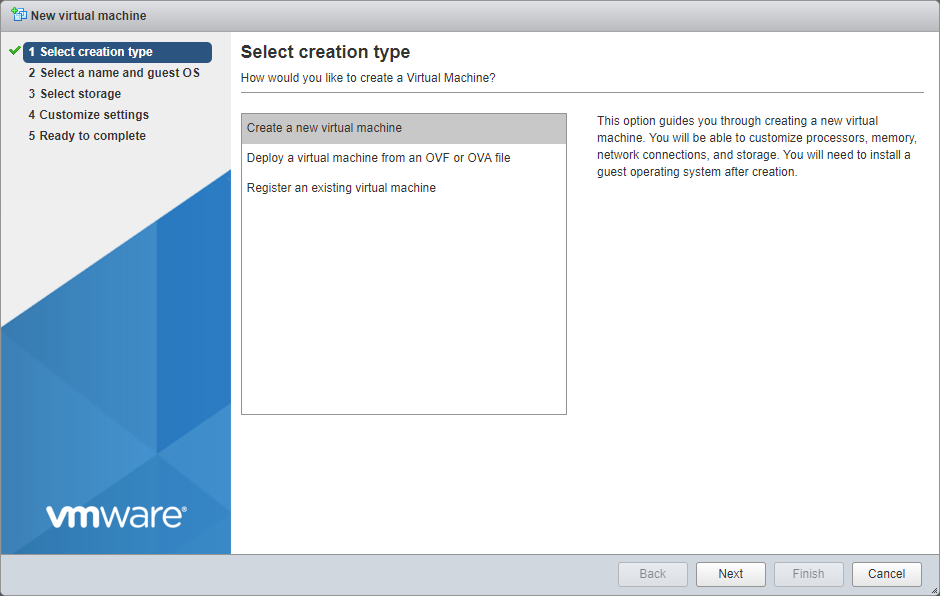
\includegraphics[width=\textwidth]{task2_06_winserver2016_2_dc_crop}
        %   \caption{[2] vSphere Web Client: Creating a new VM in ESXi}
        %   \label{fig:task2:vspherewc_newvm1}
        % \end{figure}
      \item Give the VM a unique (within the ESXi instance) name and set the Guest OS Family and Version to be `Windows` and `Microsoft Windows Server 2016 (64-bit)` respectively.
        \begin{figure}[H]
          \centering
          \captionsetup{skip=2pt}
          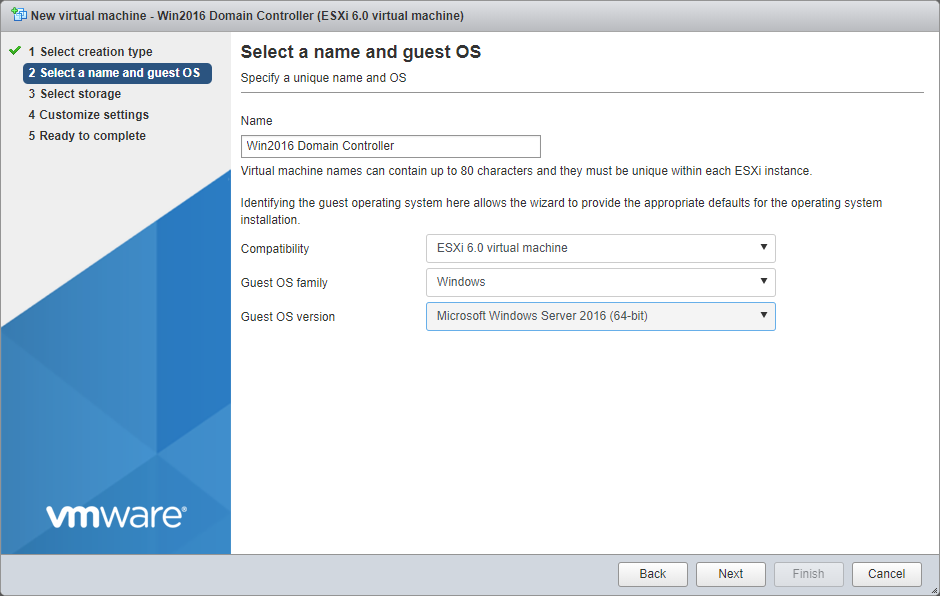
\includegraphics[width=\textwidth]{task2_06_winserver2016_3_dc_crop}
          \caption{[2] vSphere Web Client: Selecting the name and guest OS for the new VM}
          \label{fig:task2:vspherewc_newvm2}
        \end{figure}
      \item Mount the Windows Server 2016 ISO in the CD drive for the new virtual machine.
        \begin{figure}[H]
          \centering
          \captionsetup{skip=2pt}
          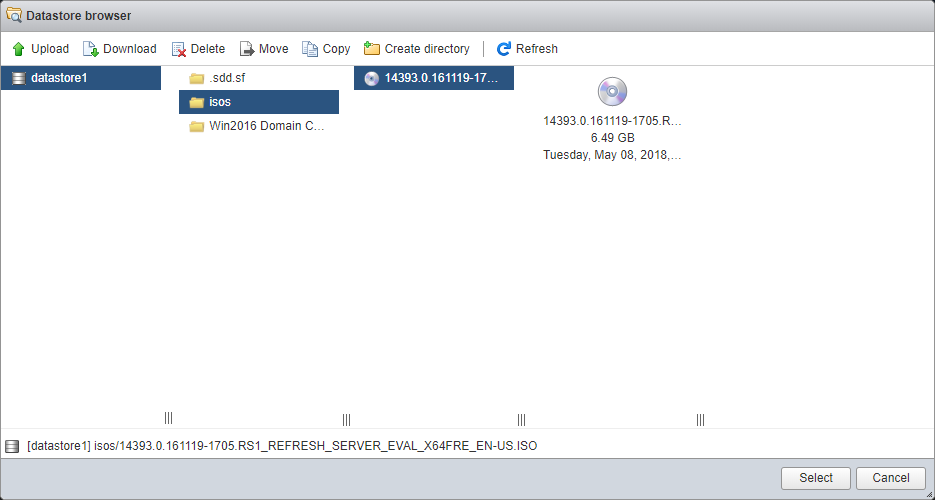
\includegraphics[width=\textwidth]{task2_06_winserver2016_9_dc_crop}
          \caption{[2] vSphere Web Client: Selecting the ISO to run at boot in the new VM}
          \label{fig:task2:vspherewc_newvm3}
        \end{figure}
    \end{enumerate}
\end{enumerate}

\noindent The screenshot in Figure~\ref{fig:task2:vspherewc_newvm4} in the \nameref{app:ancillaryscreenshots} appendix shows the Web Client UI display for the newly created VM.\\\\
\noindent For the next steps, I used the vSphere Client to display the console of specific VMs inside ESXi. This is primarily because of a bug in ESXi 6.0 that prevents consoles from being shown in the browser, as shown in Figures~\ref{fig:task2:vspherewc_bug1} and~\ref{fig:task2:vspherewc_bug2} in the \nameref{app:ancillaryscreenshots} appendix. However, the vSphere Client is also nicer to use as it responds faster and does not attempt to scale the console to the size of the browser window.

\begin{enumerate}[resume*=task2methodology2]
  \item Open a console in the vSphere Client (desktop) to the newly created VM for Windows and start it.
  \item Install Windows Server in the VM. Notable steps include:
    \begin{enumerate}[label=(\alph*)]
      \item Choosing `Windows Server 2016 Datacenter Evaluation (Desktop Experience)' edition as shown in the image below. This is done to ensure that the full feature set required for the project is included in the installation and that a desktop is available to make the server easier to configure.
        \begin{figure}[H]
          \centering
          \captionsetup{skip=2pt}
          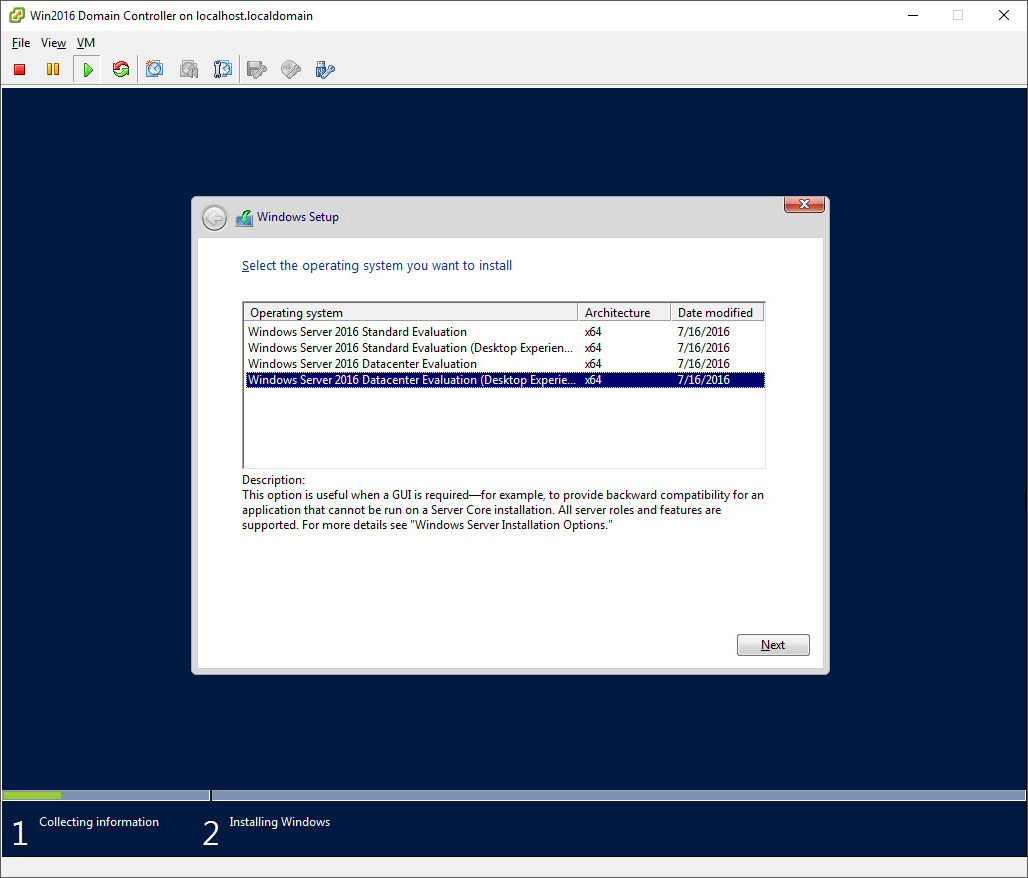
\includegraphics[width=\textwidth]{task2_6_winserver2016_15_dc}
          \caption{[2] Server 2016 Installer: Choosing `Datacenter Evaluation (Desktop Experience)'}
          \label{fig:task2:vspherec_windc1}
        \end{figure}
      \item Selecting a strong password for the administrative user. Below I have included a screenshot that shows the warning displayed in the event that the password provided does not meet the minimum complexity requirements.
        \begin{figure}[H]
          \centering
          \captionsetup{skip=2pt}
          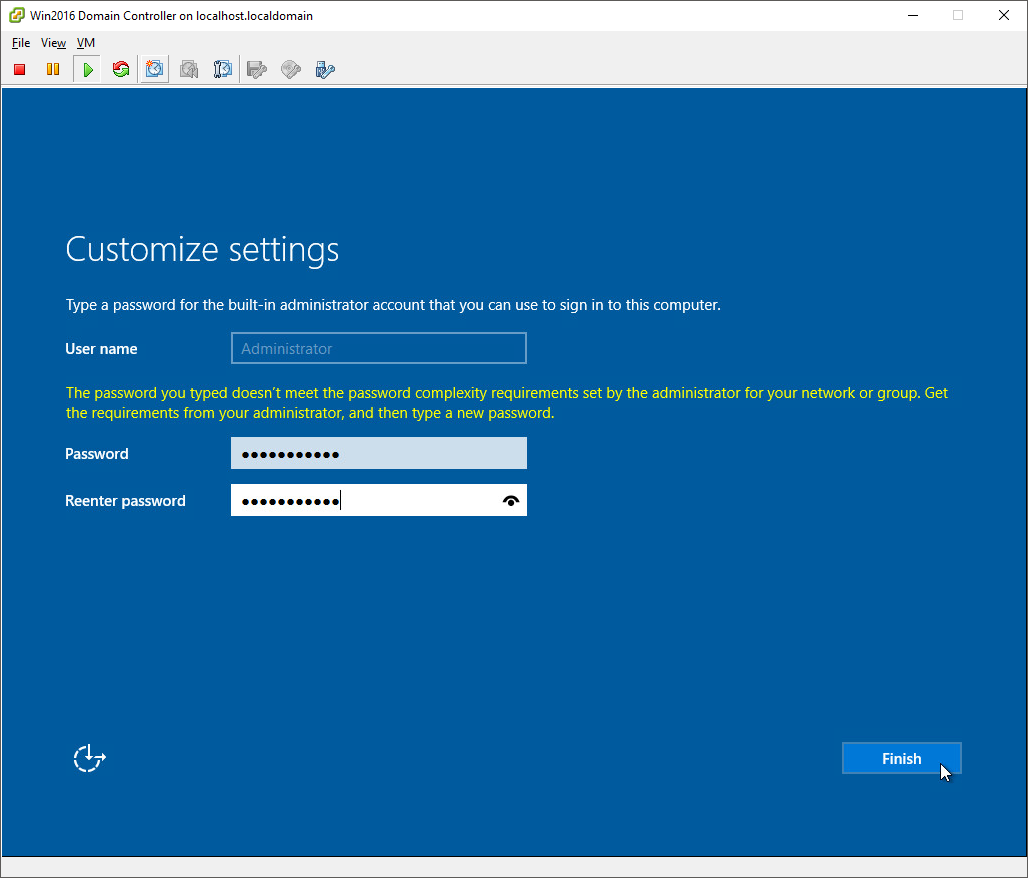
\includegraphics[width=\textwidth]{task2_6_winserver2016_21_dc}
          \caption{[2] Server 2016 Installer: Warning message displayed if password does not meet complexity requirements}
          \label{fig:task2:vspherec_windc2}
        \end{figure}
    \end{enumerate}
\end{enumerate}

% \noindent \todo{add stuff here about fixing the NAT with ESXi? and changing the hostname}

\subsubsection{Configure an Active Directory Domain Controller}
\begin{enumerate}[series=task2methodology3]
  \item Login to the Domain Controller server and in `Server Manager > Dashboard' select `Add roles and features'.
  \item Proceed through the `Add Roles and Features Wizard' as detailed in the following steps:
   \begin{enumerate}[label=(\alph*)]
     \item Select `Role-based or feature-based installation' as a this individual server is the one being configured.
       \begin{figure}[H]
         \centering
         \captionsetup{skip=2pt}
         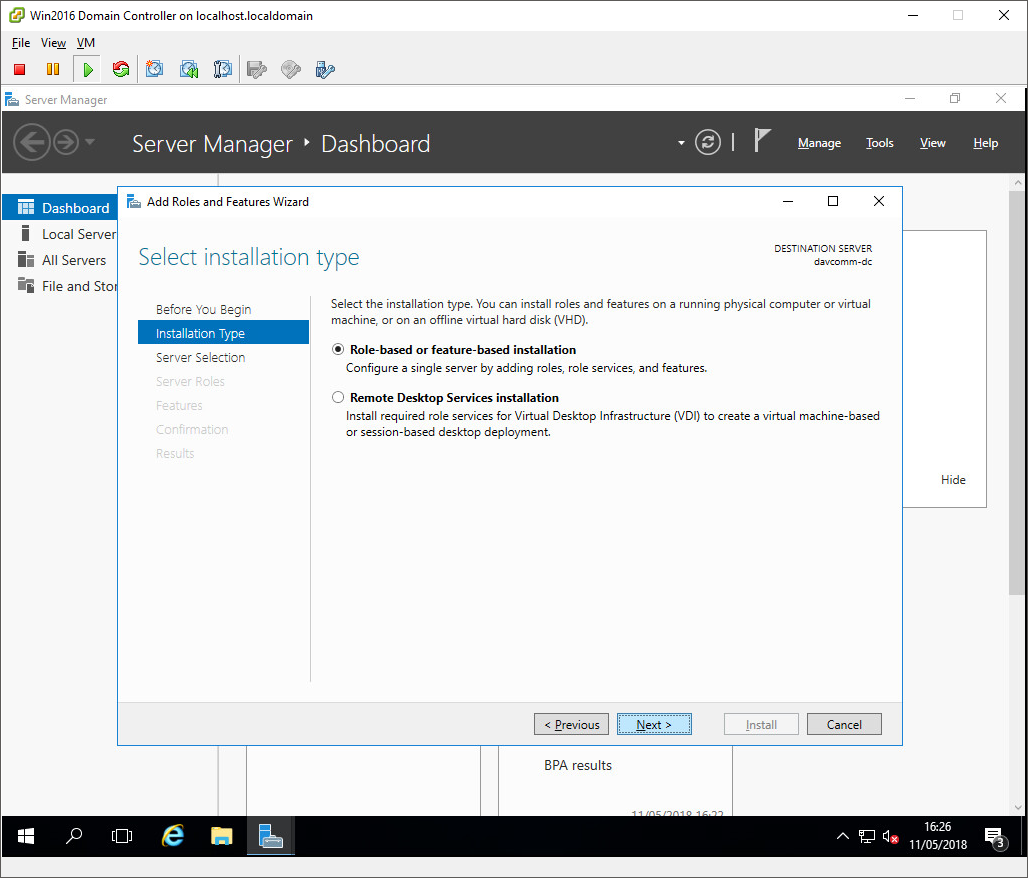
\includegraphics[width=\textwidth]{task2_6_winserver2016_25_dc_config_3}
         \caption{[2] Server 2016 DC: `Select installation type' on the Domain Controller}
         \label{fig:task2:vspherec_windc2_c3}
       \end{figure}
      \item Choose this server by its hostname.
        \begin{figure}[H]
          \centering
          \captionsetup{skip=2pt}
          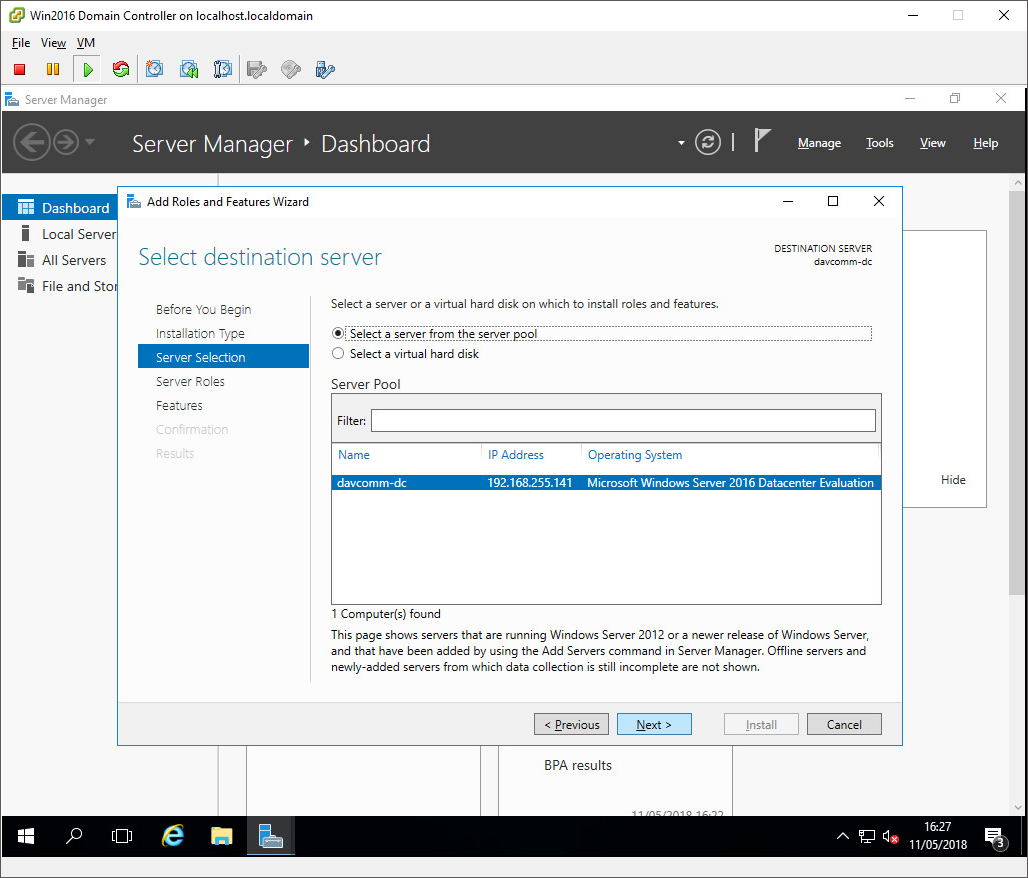
\includegraphics[width=\textwidth]{task2_6_winserver2016_25_dc_config_4}
          \caption{[2] Server 2016 DC: Selecting the server from the server pool}
          \label{fig:task2:vspherec_windc2_c4}
        \end{figure}
      \item Select the roles `Active Directory Domain Services' and `DNS Server' and confirm the addition of features for both.
        \begin{figure}[H]
          \centering
          \captionsetup{skip=2pt}
          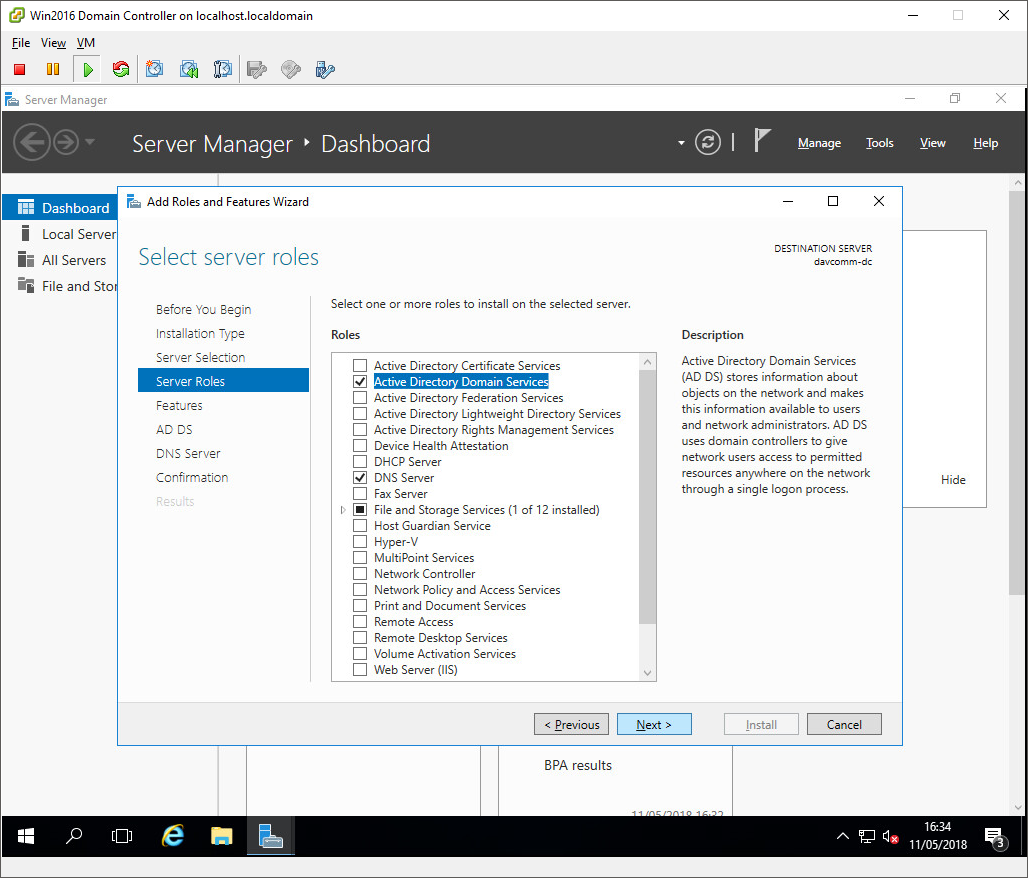
\includegraphics[width=\textwidth]{task2_6_winserver2016_25_dc_config_7}
          \caption{[2] Server 2016 DC: Select the roles `Active Directory Domain Services' and `DNS Server'}
          \label{fig:task2:vspherec_windc2_c7}
        \end{figure}
        \begin{figure}[H]
          \centering
          \captionsetup{skip=2pt}
          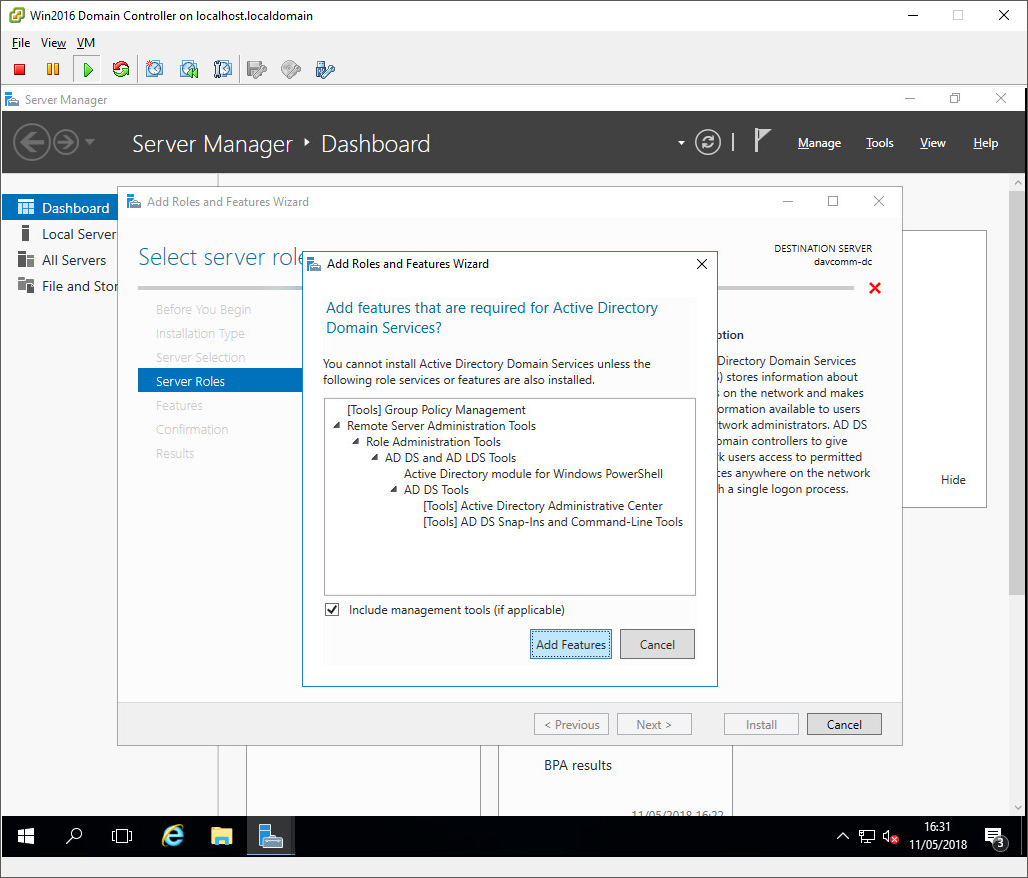
\includegraphics[width=\textwidth]{task2_6_winserver2016_25_dc_config_5}
          \caption{[2] Server 2016 DC: Add the features for `Active Directory Domain Services'}
          \label{fig:task2:vspherec_windc2_c5}
        \end{figure}
        \begin{figure}[H]
          \centering
          \captionsetup{skip=2pt}
          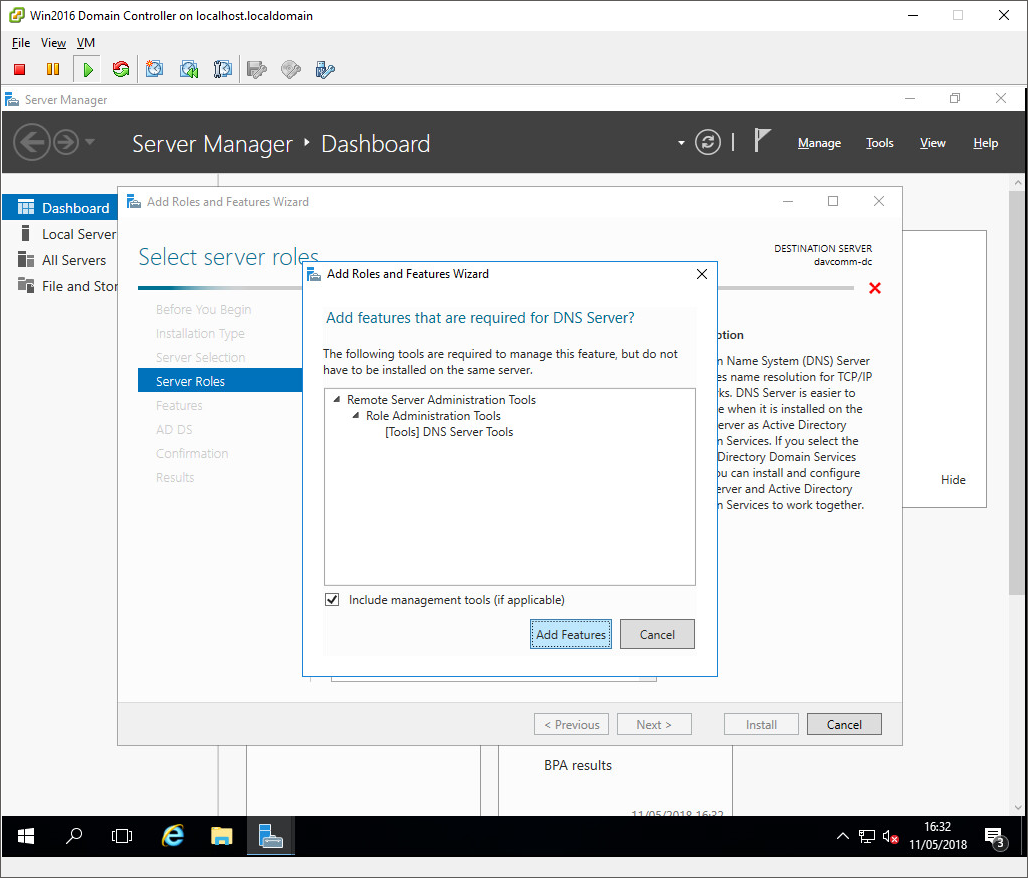
\includegraphics[width=\textwidth]{task2_6_winserver2016_25_dc_config_6}
          \caption{[2] Server 2016 DC: Add the features required for the `DNS Server' role}
          \label{fig:task2:vspherec_windc2_c6}
        \end{figure}
      \item Confirm the installation of the selected roles, selecting the option to `Restart the destination server automatically if required'.
        \begin{figure}[H]
          \centering
          \captionsetup{skip=2pt}
          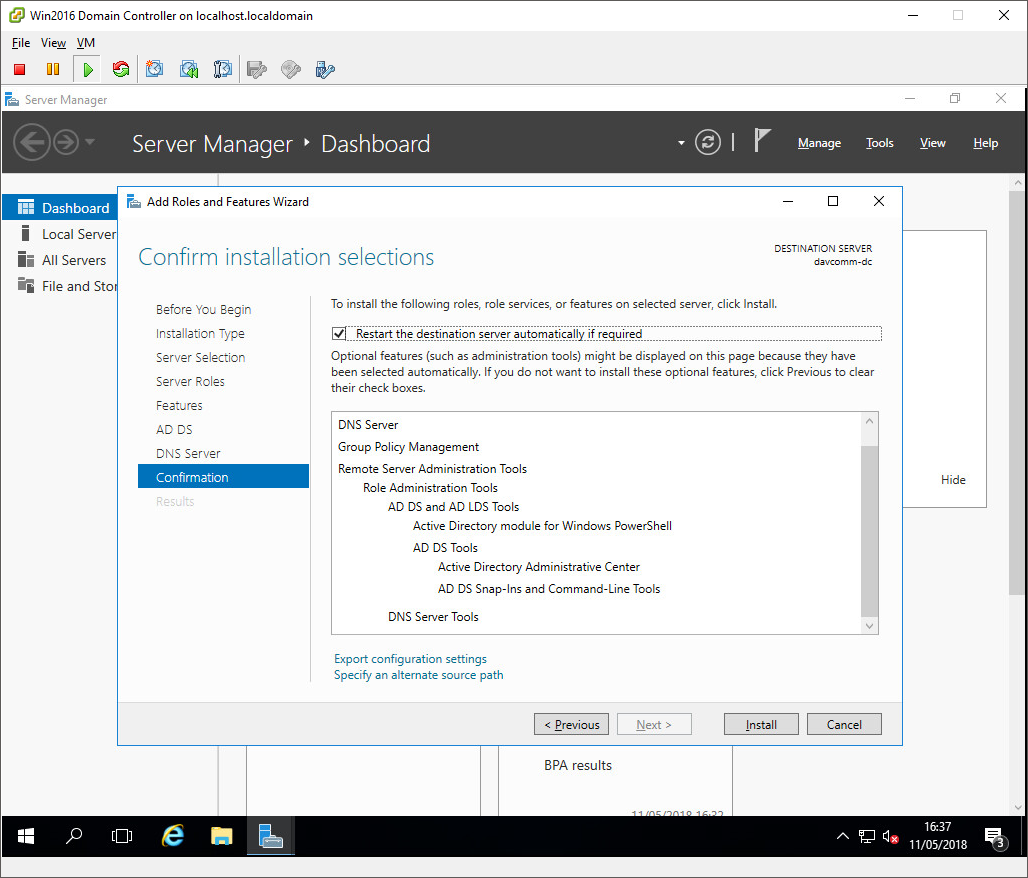
\includegraphics[width=\textwidth]{task2_6_winserver2016_25_dc_config_10}
          \caption{[2] Server 2016 DC: Confirm the installation by selecting `Install'}
          \label{fig:task2:vspherec_windc2_c10}
        \end{figure}
      \item Create a new forest for the ADDS Deployment Configuration by selecting `Add a new forest' and giving a qualified domain name.
        \begin{figure}[H]
          \centering
          \captionsetup{skip=2pt}
          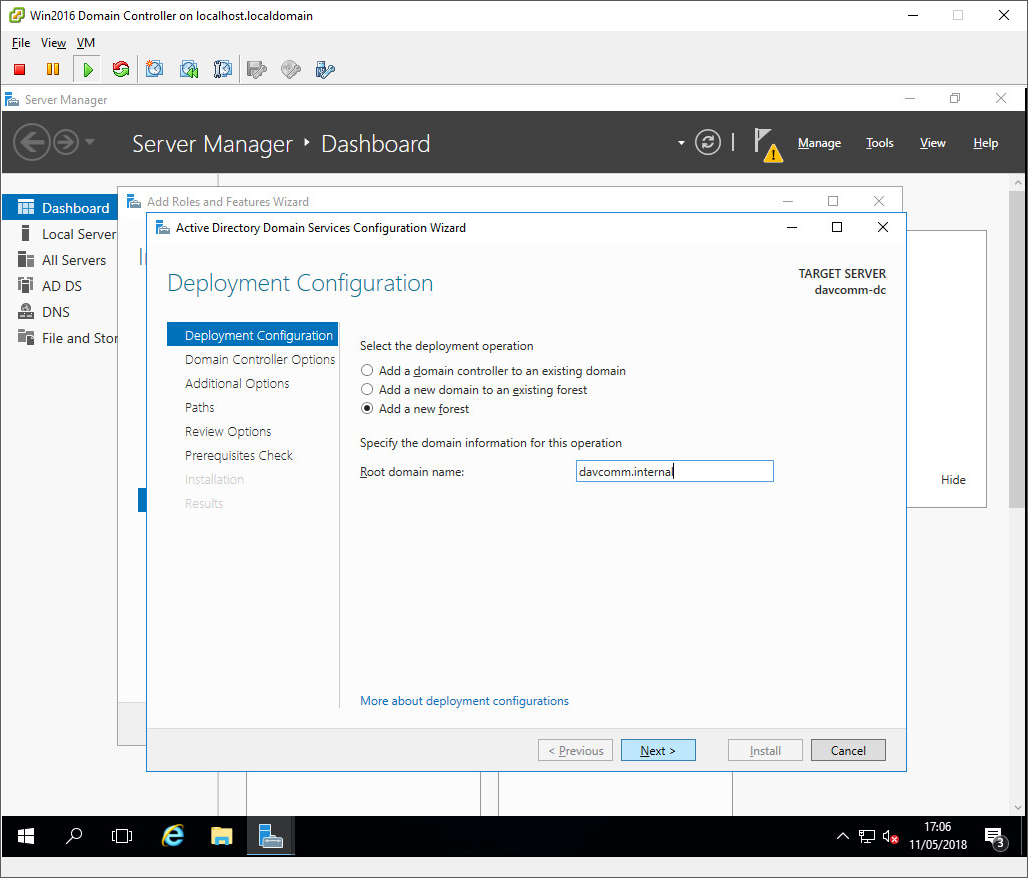
\includegraphics[width=\textwidth]{task2_6_winserver2016_25_dc_config_13}
          \caption{[2] Server 2016 DC: Create a new forest for the domain}
          \label{fig:task2:vspherec_windc2_c13}
        \end{figure}
      \item Configure the `Domain Controller Options' -- as there are no servers in this deployment older than Windows Server 2016, select that as the functional level. Choose a strong password for the `Directory Services Restore Mode' password.
        \begin{figure}[H]
          \centering
          \captionsetup{skip=2pt}
          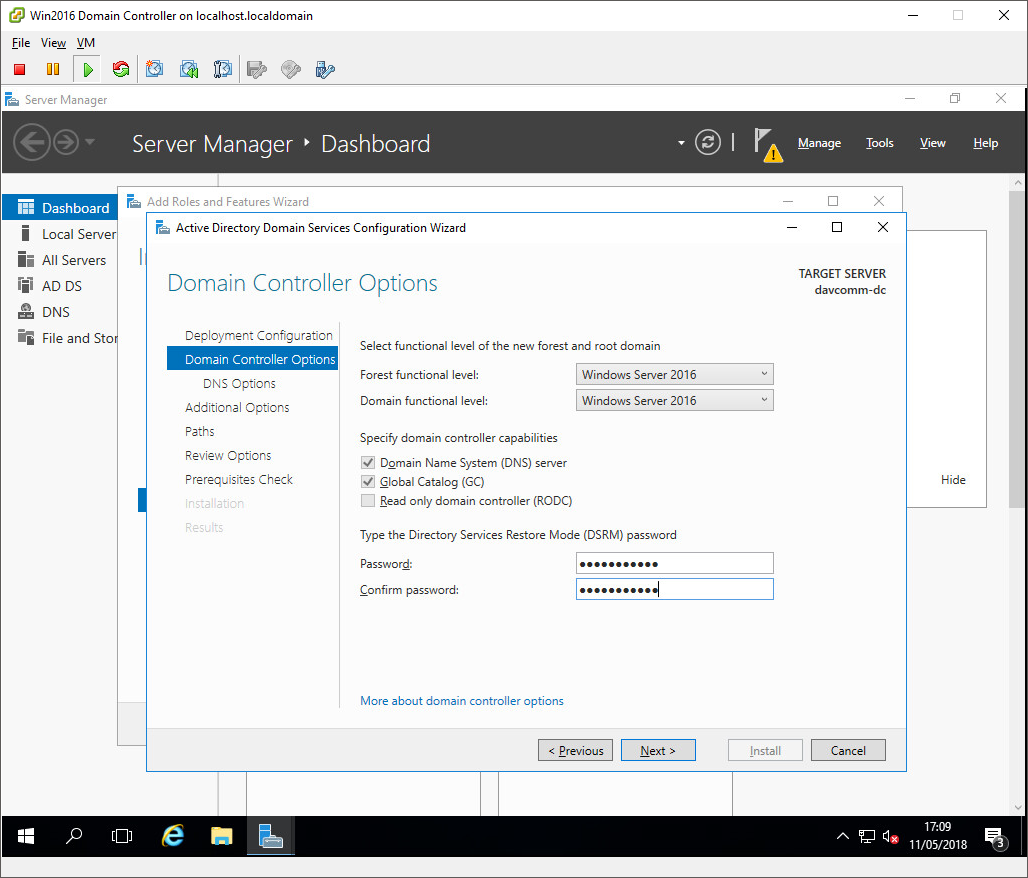
\includegraphics[width=\textwidth]{task2_6_winserver2016_25_dc_config_14}
          \caption{[2] Server 2016 DC: Configuring options for the Domain Controller}
          \label{fig:task2:vspherec_windc2_c14}
        \end{figure}
      \item As this is an internal deployment, an authoritative parent zone for the DNS cannot be found. Therefore ignore this warning step for `DNS Options' by selecting Next.
        \begin{figure}[H]
          \centering
          \captionsetup{skip=2pt}
          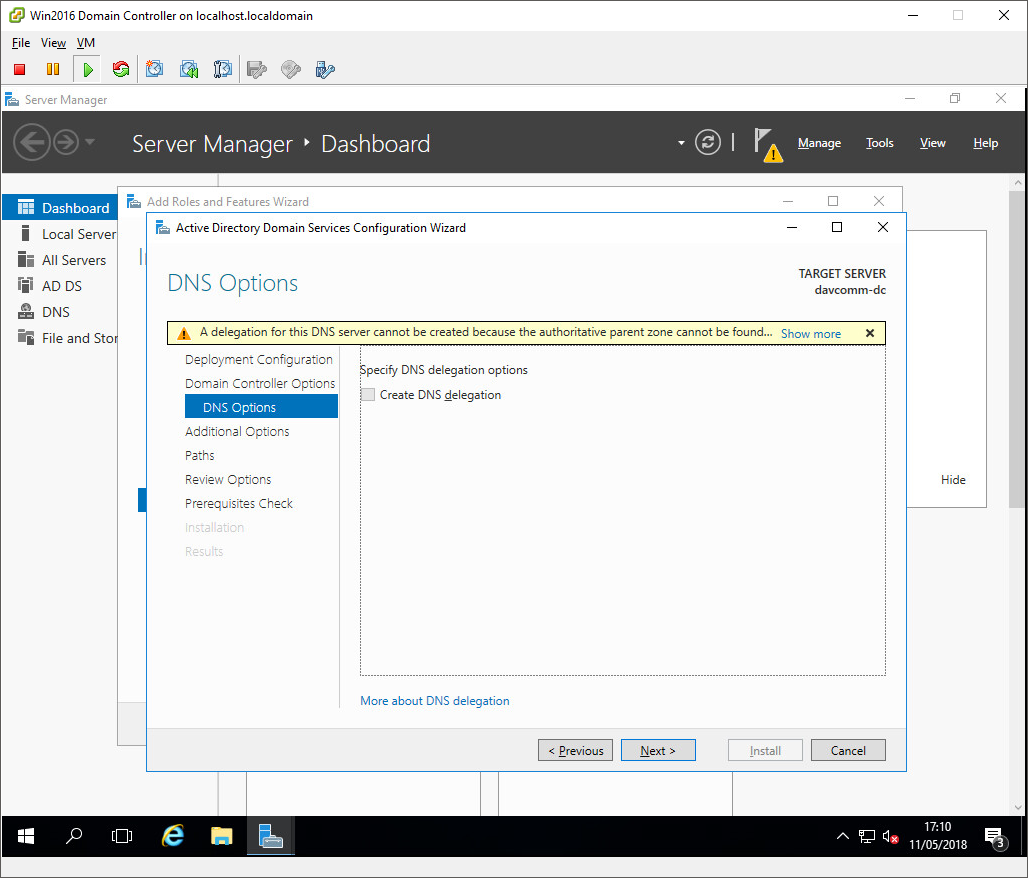
\includegraphics[width=\textwidth]{task2_6_winserver2016_25_dc_config_15}
          \caption{[2] Server 2016 DC: DNS Options delegation warning}
          \label{fig:task2:vspherec_windc2_c15}
        \end{figure}
      \item Set the NetBIOS name that should be assigned to the domain.
        \begin{figure}[H]
          \centering
          \captionsetup{skip=2pt}
          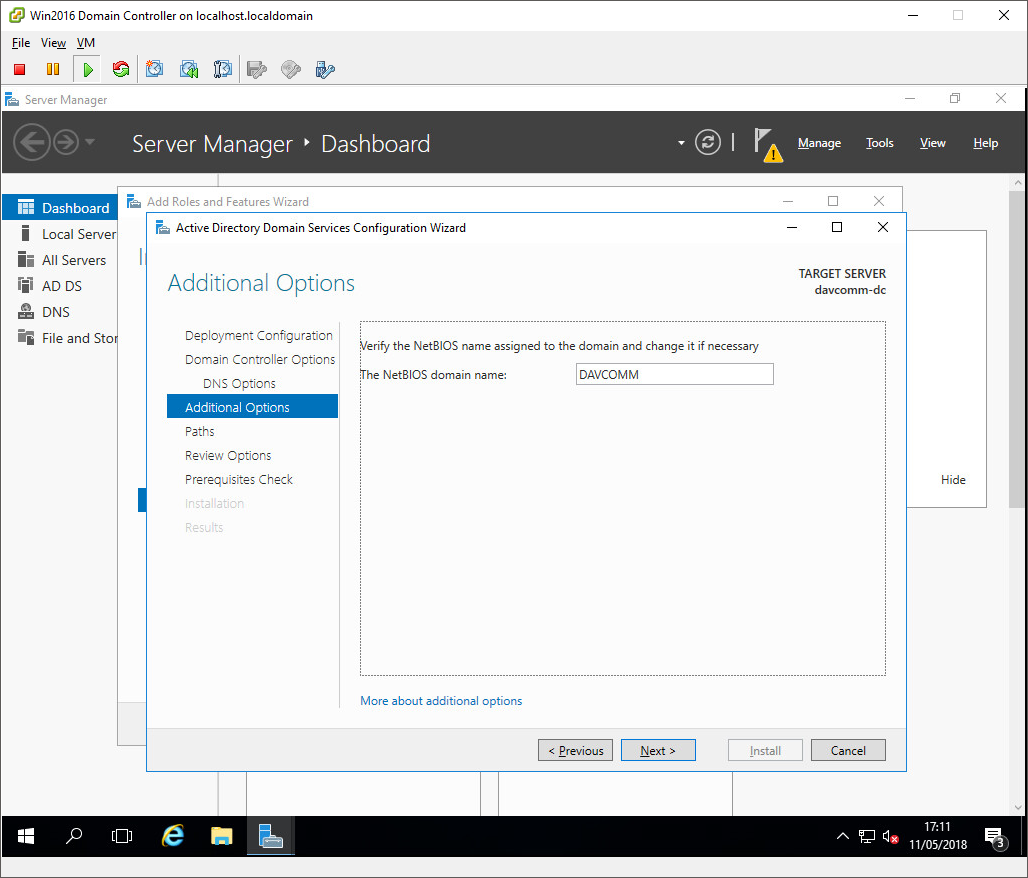
\includegraphics[width=\textwidth]{task2_6_winserver2016_25_dc_config_16}
          \caption{[2] Server 2016 DC: Setting the NetBIOS name}
          \label{fig:task2:vspherec_windc2_c16}
        \end{figure}
      \item In the `Paths' step, click Next to accept the default options that are provided. Here we could choose to store the log files in a different partition (to prevent them from filling the C drive in the event that a lot of log files are created accidentally as a result of a misconfiguration) or on a remote logging server (for increased security -- by backing up the logs on the logging server regularly and/or watching attempts to modify logs via a firewall).
        \begin{figure}[H]
          \centering
          \captionsetup{skip=2pt}
          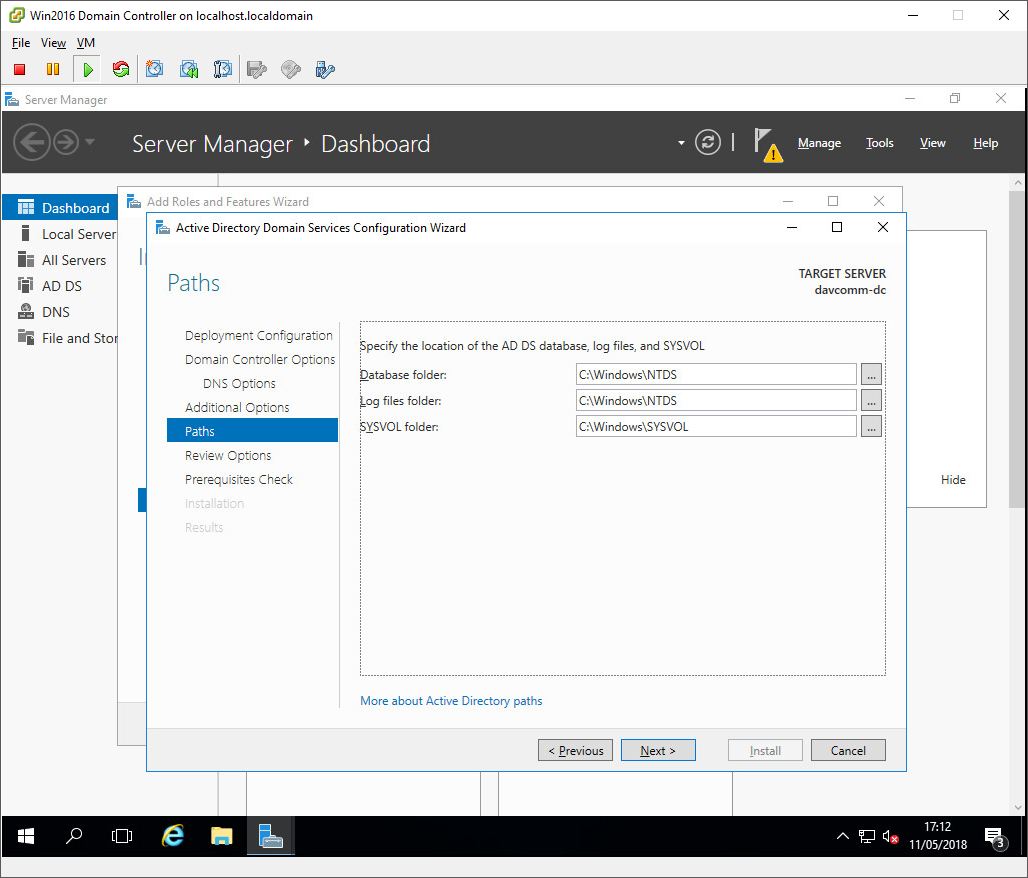
\includegraphics[width=\textwidth]{task2_6_winserver2016_25_dc_config_17}
          \caption{[2] Server 2016 DC: Accept the default `Paths' for the ADDS configuration}
          \label{fig:task2:vspherec_windc2_c17}
        \end{figure}
      \item Review the options selected throughout the configuration to confirm that the correct options have been selected at each stage. Notable here is the ability to view a PowerShell script, as shown in Figure~\ref{fig:task2:vspherec_windc2_c19}. PowerShell scripts could be used to automate the deployment of new servers when not using the Desktop Experience version of Windows Server 2016.
        \begin{figure}[H]
          \centering
          \captionsetup{skip=2pt}
          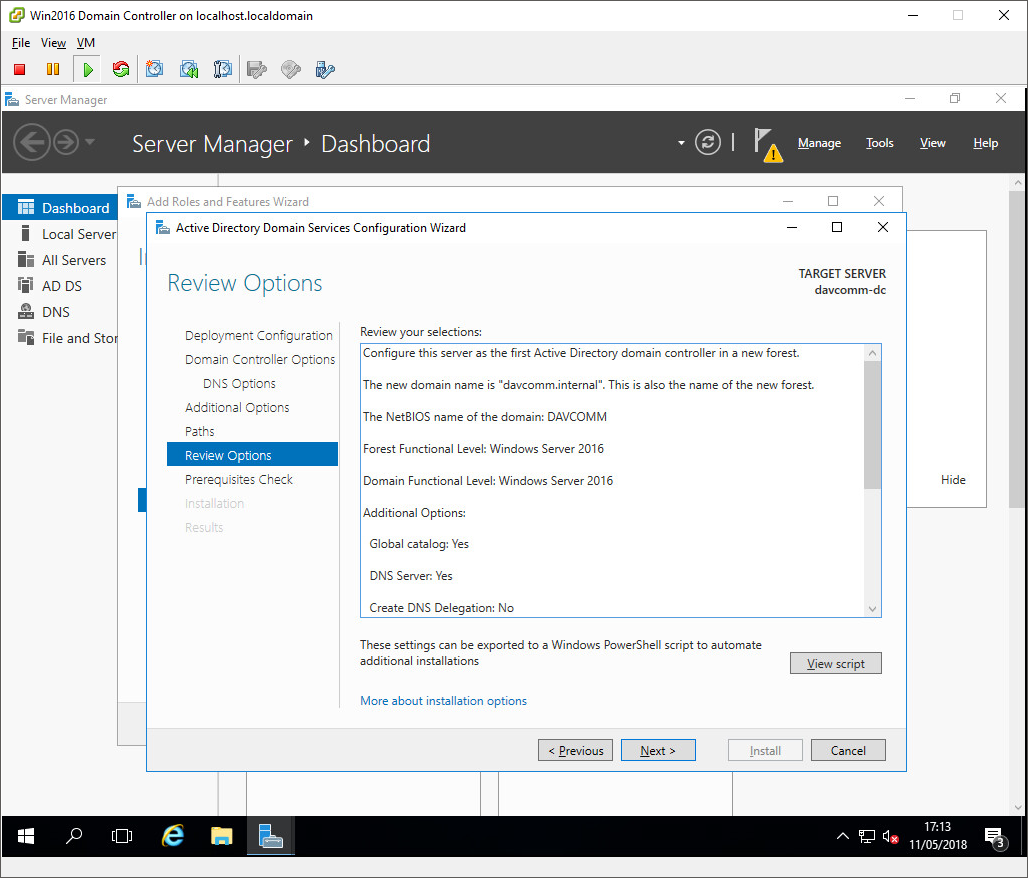
\includegraphics[width=\textwidth]{task2_6_winserver2016_25_dc_config_18}
          \caption{[2] Server 2016 DC: Review the options for the Domain Controller configuration}
          \label{fig:task2:vspherec_windc2_c18}
        \end{figure}
        \begin{figure}[H]
          \centering
          \captionsetup{skip=2pt}
          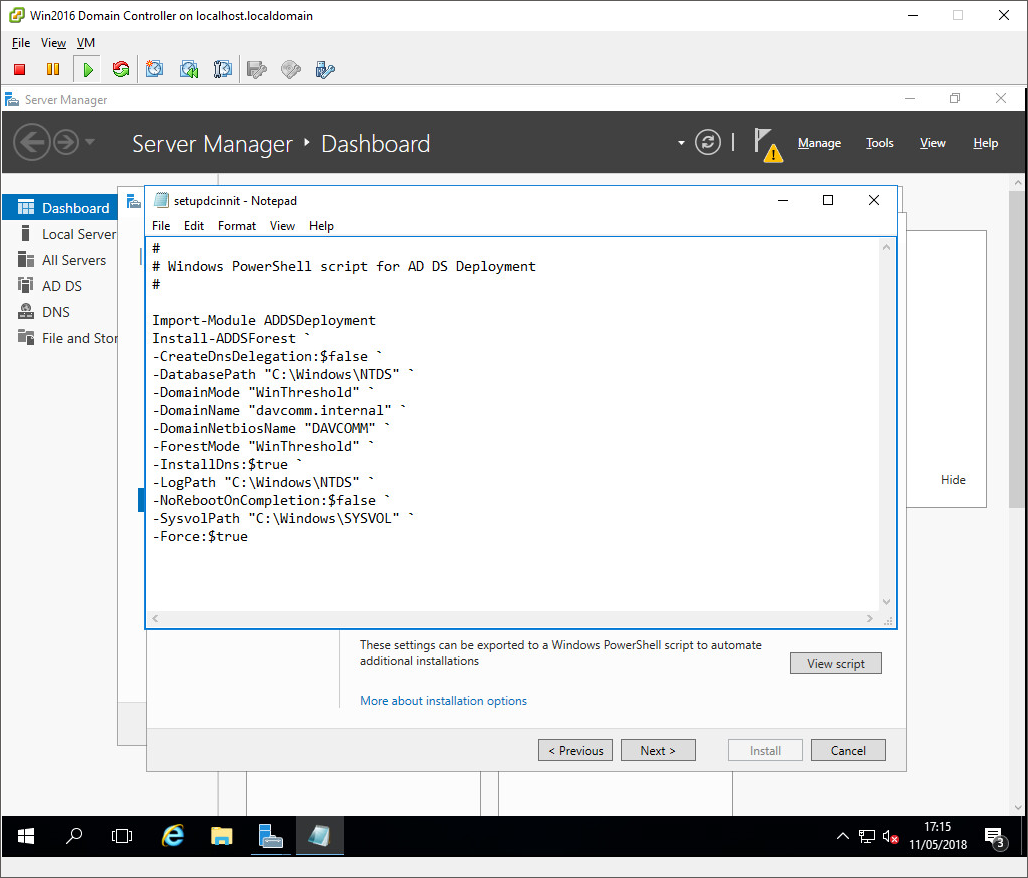
\includegraphics[width=\textwidth]{task2_6_winserver2016_25_dc_config_19}
          \caption{[2] Server 2016 DC: PowerShell script for the DC configuration}
          \label{fig:task2:vspherec_windc2_c19}
        \end{figure}
      \item Finally, review the `Prerequisites Check` step. We can see from the screenshot that all checked passed successfully. Select `Install' to complete the addition of the ADDS role.
        \begin{figure}[H]
          \centering
          \captionsetup{skip=2pt}
          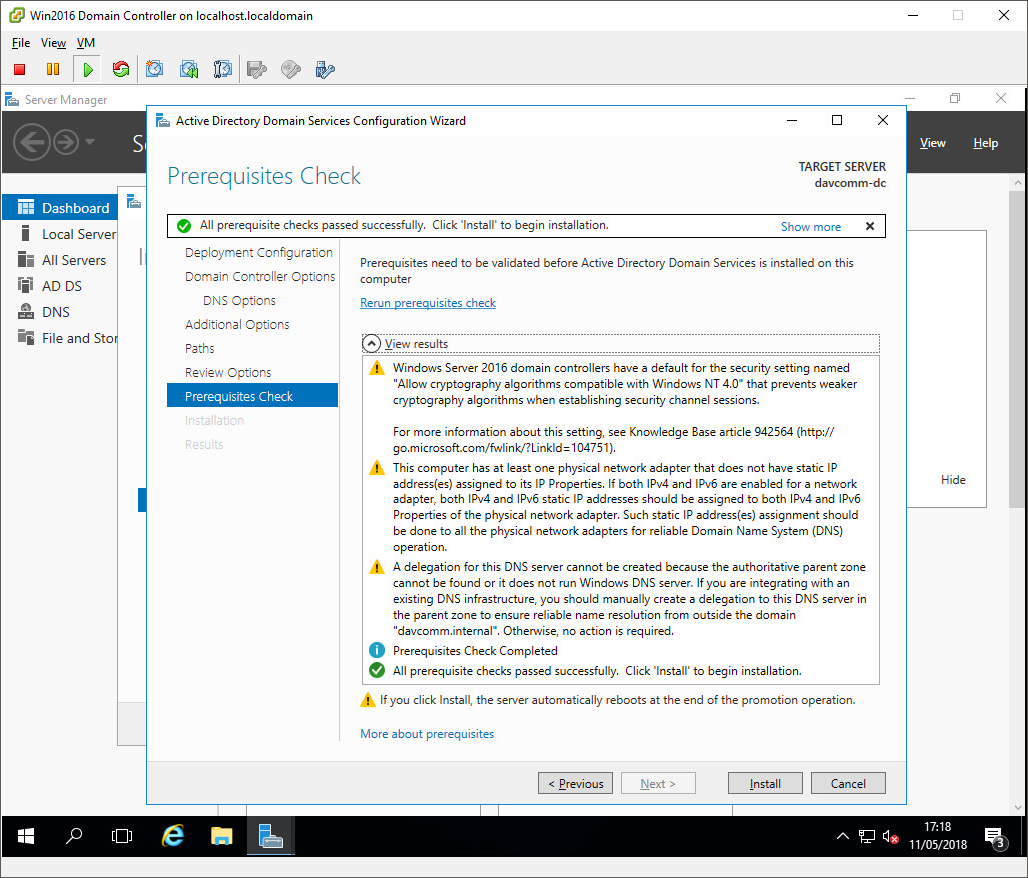
\includegraphics[width=\textwidth]{task2_6_winserver2016_25_dc_config_20}
          \caption{[2] Server 2016 DC: Active Directory Domain Services Prerequisites Check step}
          \label{fig:task2:vspherec_windc2_c20}
        \end{figure}
      \item After the server has completed installation of Active Directory Domain Services and restarted automatically, login to the Administrator account as part of the new `DAVCOMM' domain.
        \begin{figure}[H]
          \centering
          \captionsetup{skip=2pt}
          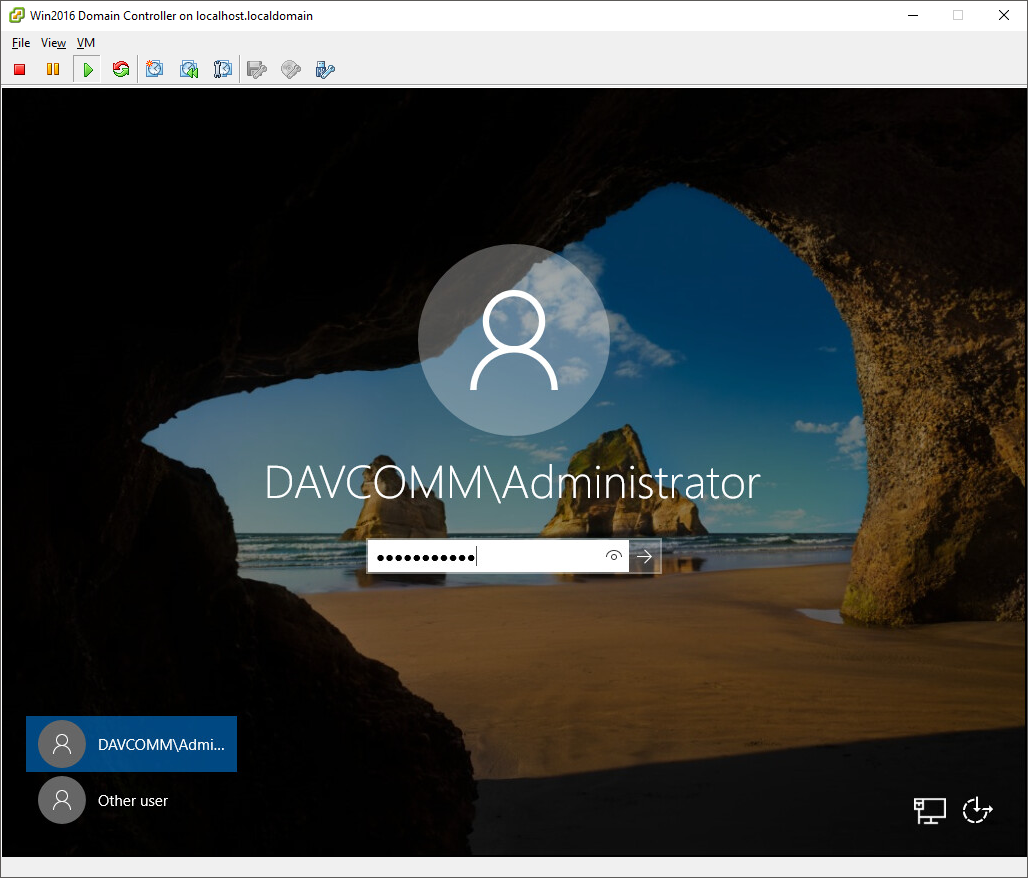
\includegraphics[width=\textwidth]{task2_6_winserver2016_25_dc_config_21}
          \caption{[2] Server 2016 DC: Logging into the DAVCOMM\textbackslash Administrator account}
          \label{fig:task2:vspherec_windc2_c21}
        \end{figure}
      \item Check that the preferred DNS server address is set to 127.0.0.1 (this Domain Controller machine itself). This shows that the DNS Server role was installed and configured correctly. At this stage, also set the IP Address to be Static. This is done to ensure that we can consistently point the `Preferred DNS server' address of other servers and clients in the domain at the Domain Controller.
        \begin{figure}[H]
          \centering
          \captionsetup{skip=2pt}
          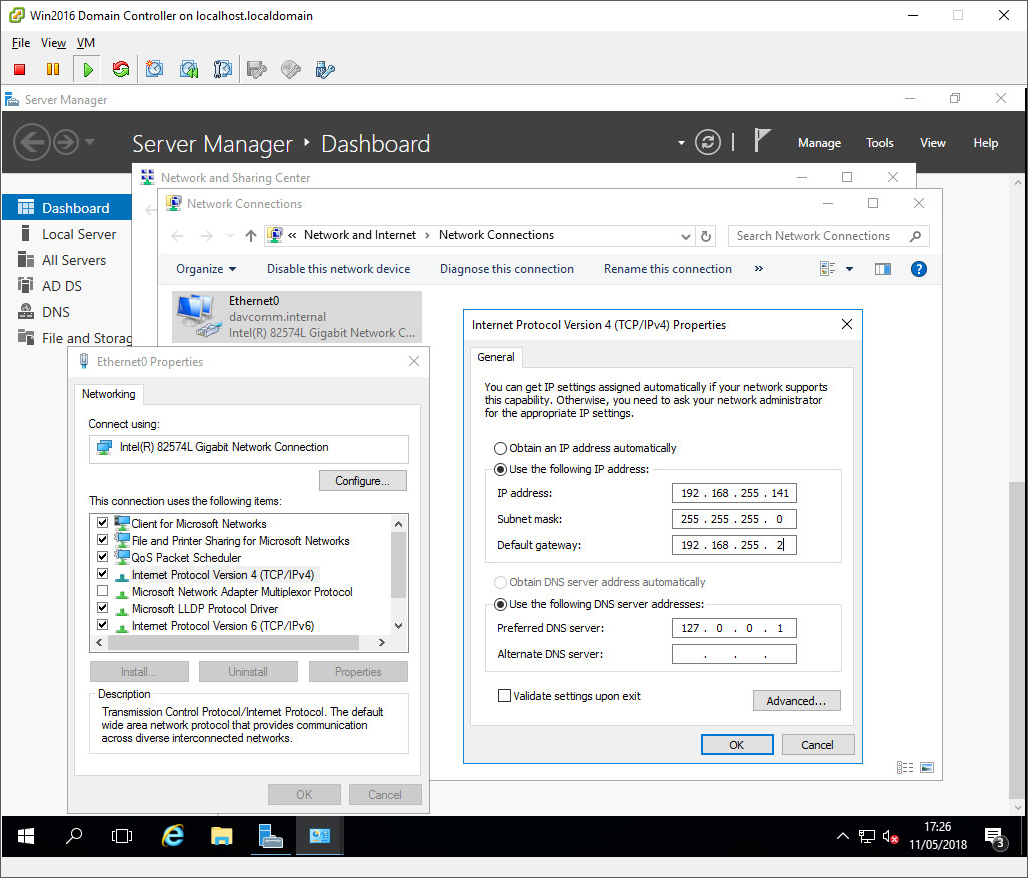
\includegraphics[width=\textwidth]{task2_6_winserver2016_25_dc_config_22_adjustipdns}
          \caption{[2] Server 2016 DC: Configuring a static IP and verifying DNS configuration}
          \label{fig:task2:vspherec_windc2_c22}
        \end{figure}
   \end{enumerate}
\end{enumerate}


\subsubsection{Set up a User Server}
The majority of the process for setting up the user server, in terms of creating a new VM in ESXi and installing Windows Server 2016, uses the same methodology of that of the Domain Controller server. I will skip the detail for these steps and only include screenshots reviewing the process in the interest of brevity.
\begin{enumerate}[series=task2methodology4]
  \item Setup a new VM in ESXi for the User Server.
    \begin{figure}[H]
      \centering
      \captionsetup{skip=2pt}
      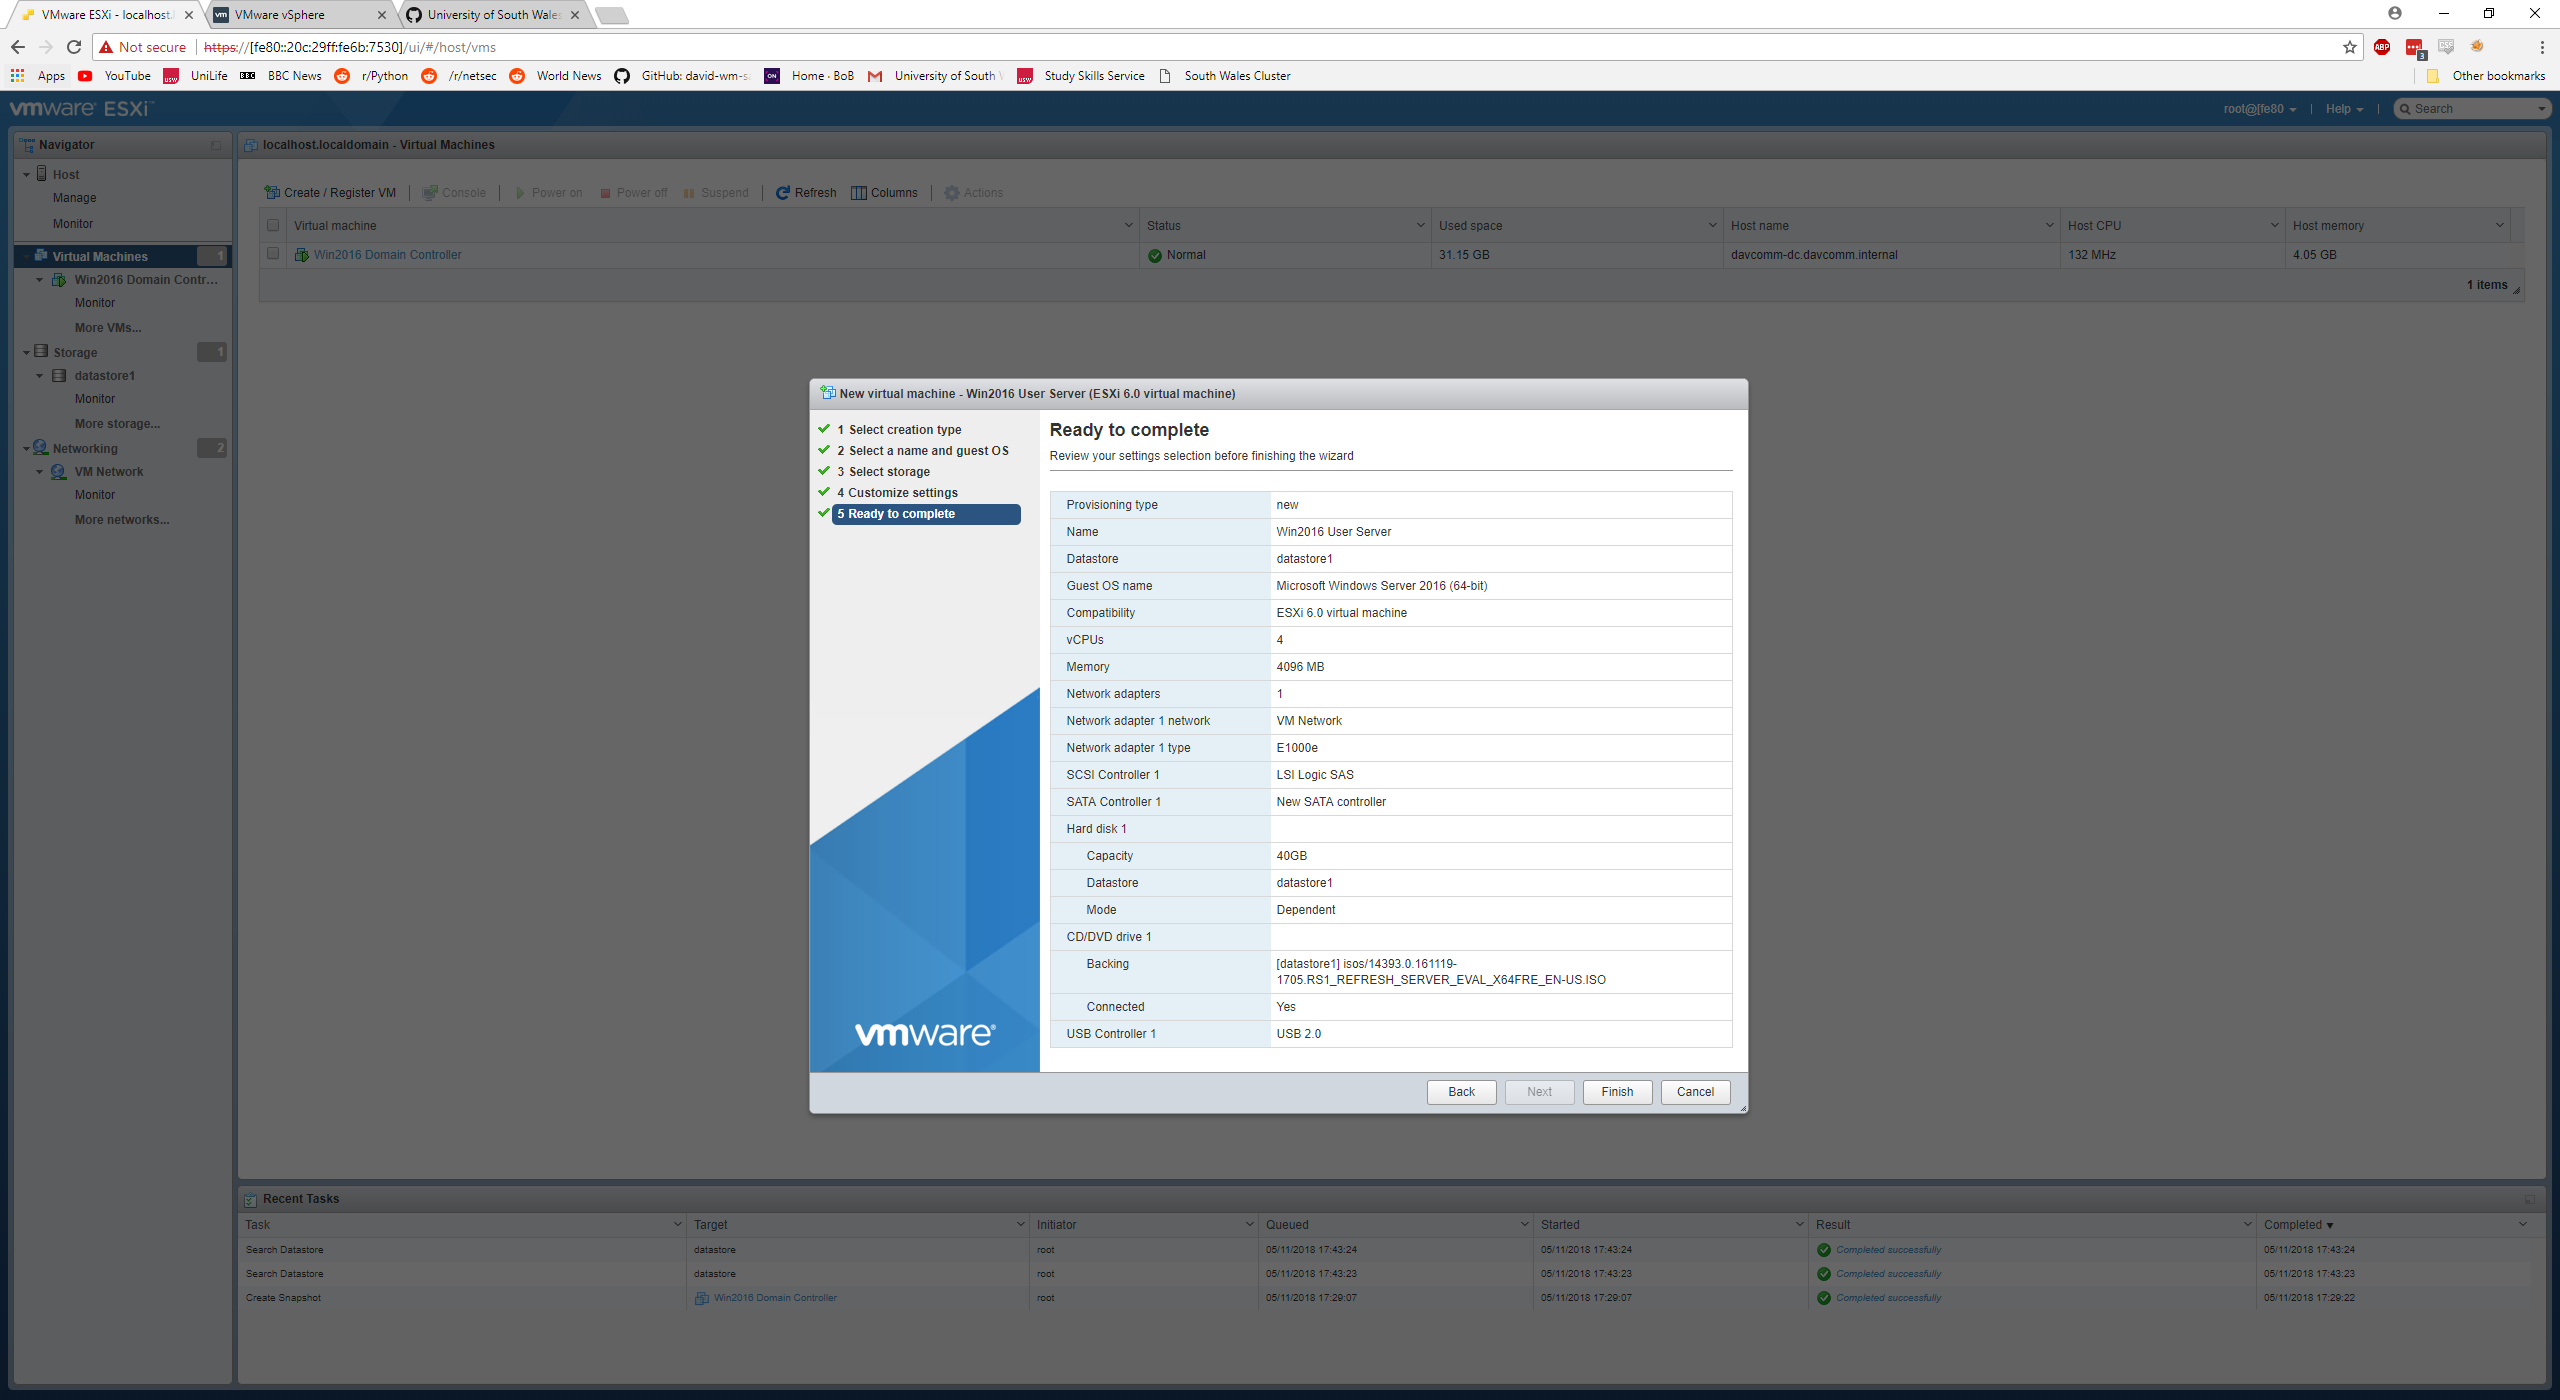
\includegraphics[width=\textwidth]{task2_9_winserver2016us_1}
      \caption{[2] vSphere Web Client: Reviewing User Server VM options in ESXi WebUI}
      \label{fig:task2:vspherec_us1}
    \end{figure}
  \item After installing the User Server, point the DNS to the static IP of the Domain Controller.
    \begin{figure}[H]
      \centering
      \captionsetup{skip=2pt}
      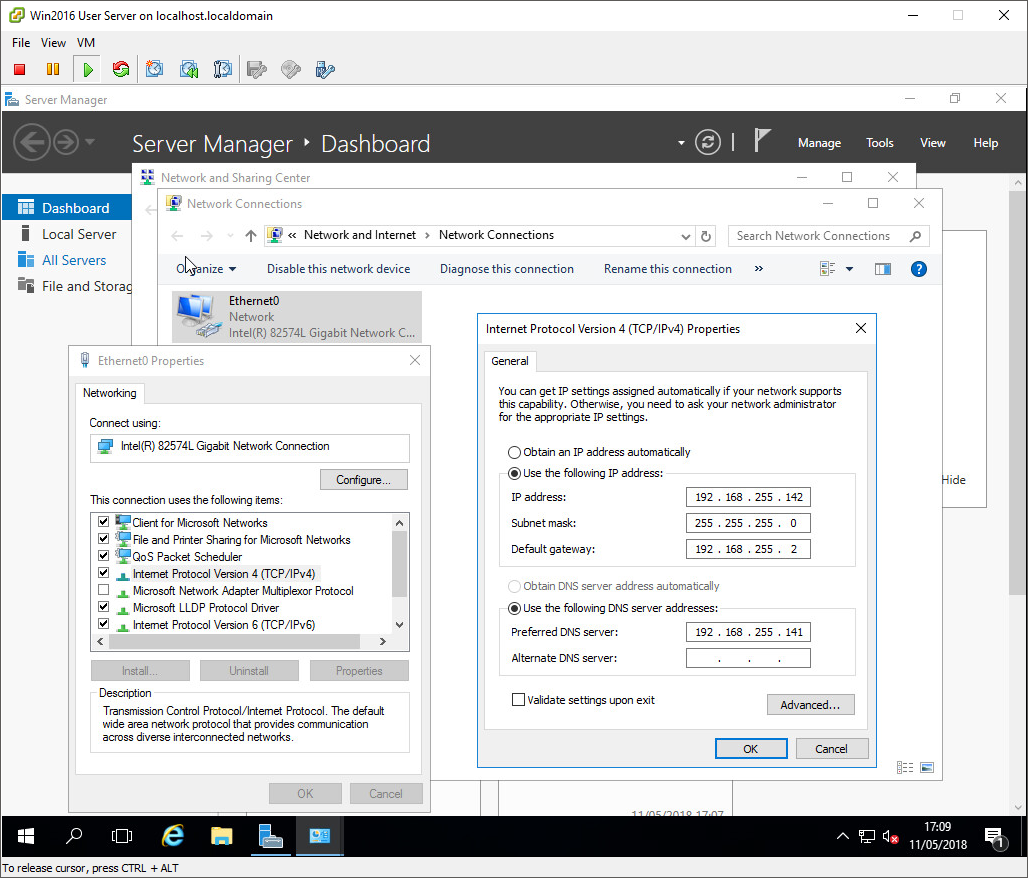
\includegraphics[width=\textwidth]{task2_9_winserver2016us_2}
      \caption{[2] Server 2016 US: Changing the `Preferred DNS server'}
      \label{fig:task2:vspherec_us2}
    \end{figure}
  \item Confirm that the previous step has worked successfully by pinging the Domain Controller.
    \begin{figure}[H]
      \centering
      \captionsetup{skip=2pt}
      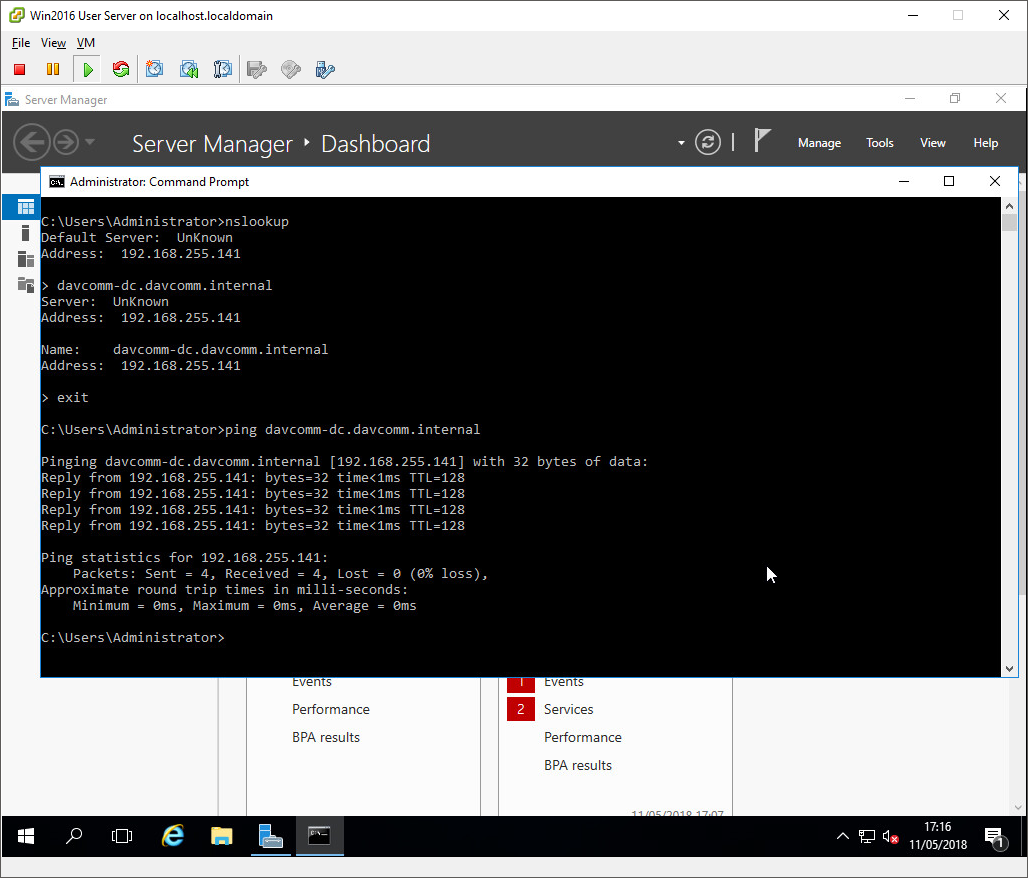
\includegraphics[width=\textwidth]{task2_9_winserver2016us_3}
      \caption{[2] Server 2016 US: Checking that the User Server can see the DC}
      \label{fig:task2:vspherec_us3}
    \end{figure}
  \item Change the hostname of the User Server and connect to the domain at the same time.
    \begin{figure}[H]
      \centering
      \captionsetup{skip=2pt}
      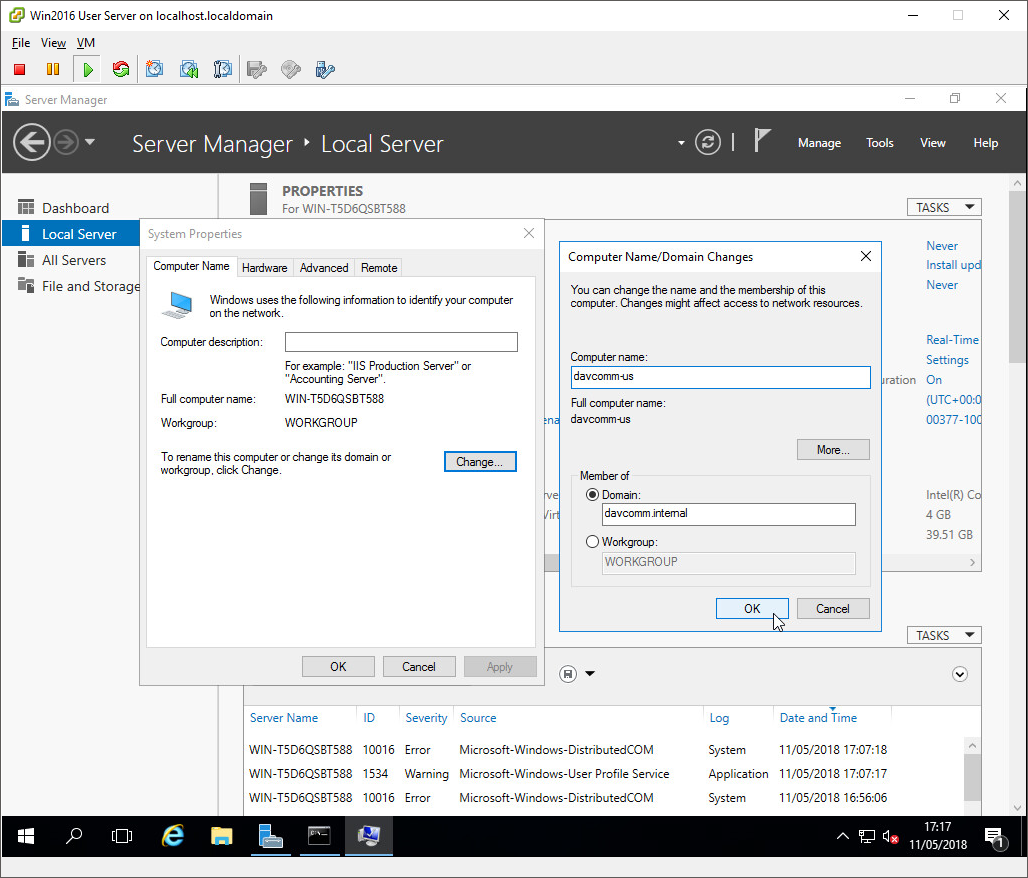
\includegraphics[width=\textwidth]{task2_9_winserver2016us_4}
      \caption{[2] Server 2016 US: Connecting to the domain}
      \label{fig:task2:vspherec_us4}
    \end{figure}
  \item After authenticating with the domain, using the username and password of the Administrator account on the Domain Controller, we can see that we have joined the domain successfully.
    \begin{figure}[H]
      \centering
      \captionsetup{skip=2pt}
      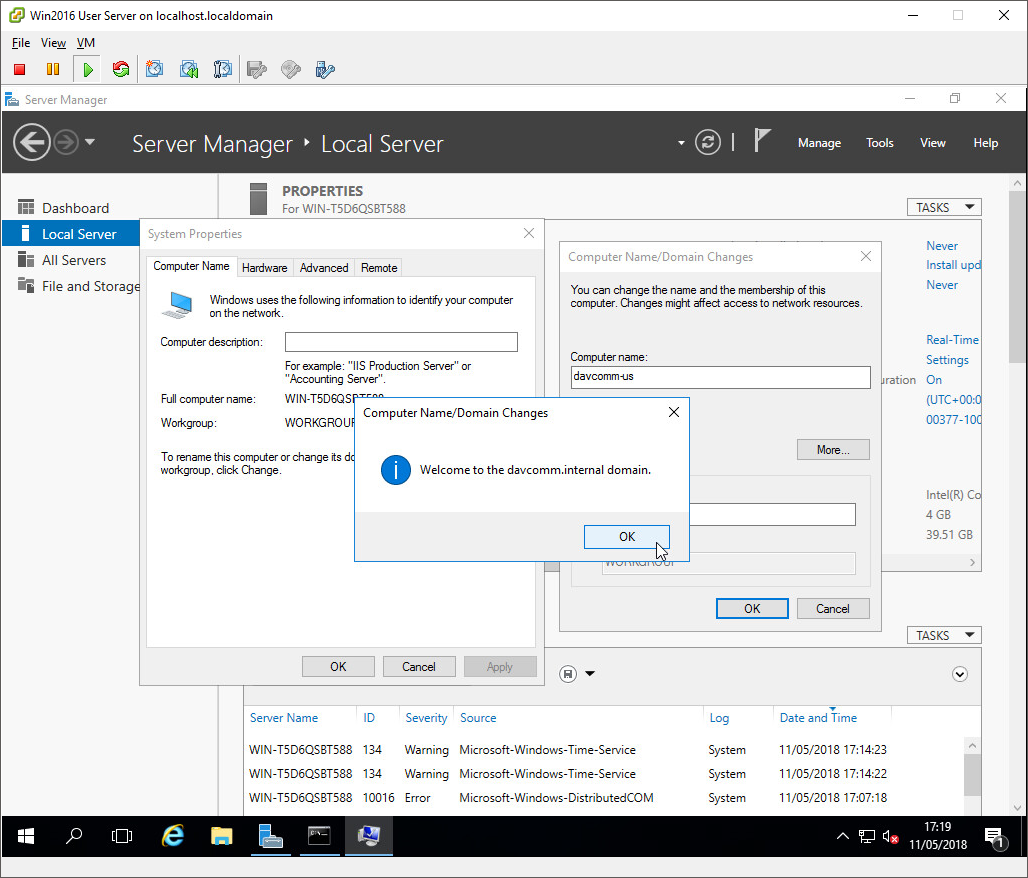
\includegraphics[width=\textwidth]{task2_9_winserver2016us_5}
      \caption{[2] Server 2016 US: `Welcome to the davcomm.internal domain' popup}
      \label{fig:task2:vspherec_us5}
    \end{figure}
  \item Restart the User Server to confirm the change to the hostname and then login to the domain.
    \begin{figure}[H]
      \centering
      \captionsetup{skip=2pt}
      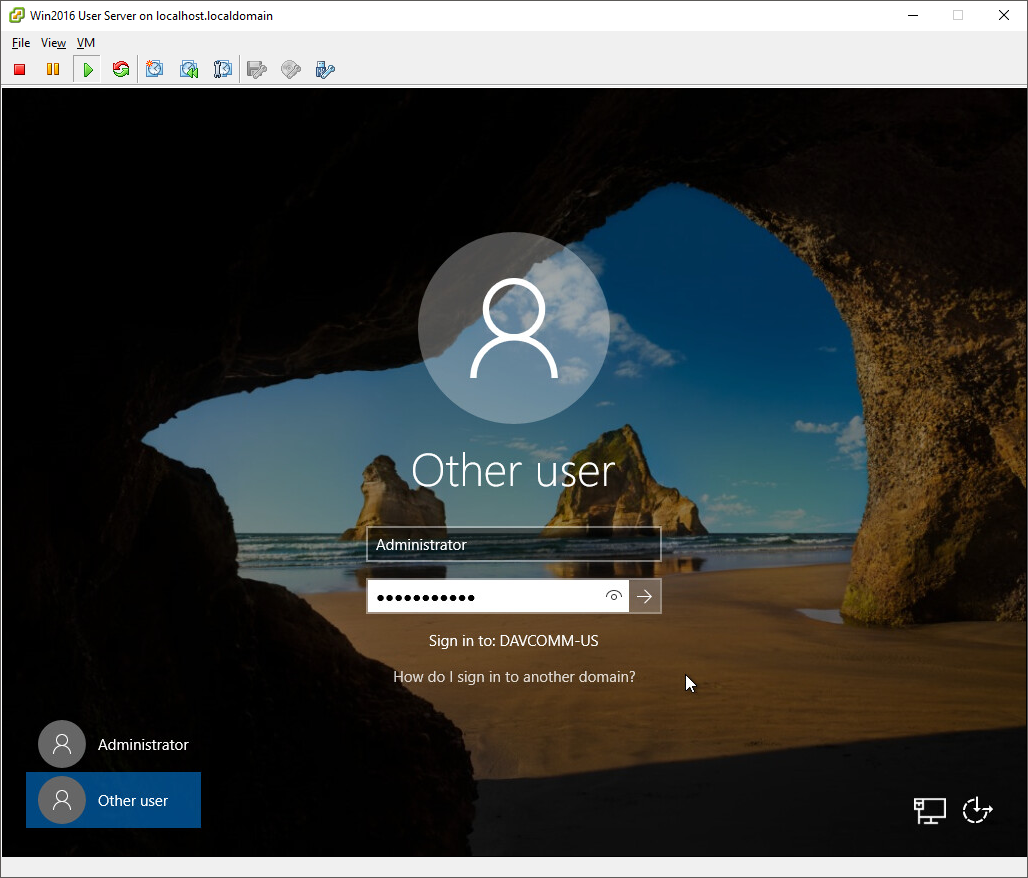
\includegraphics[width=\textwidth]{task2_9_winserver2016us_7}
      \caption{[2] Server 2016 US: Logging into the domain on the User Server}
      \label{fig:task2:vspherec_us7}
    \end{figure}
  % \item \todo{after installing vmware tools we see this in the vsphere webui}
  %   \begin{figure}[H]
  %     \centering
  %     \captionsetup{skip=2pt}
  %     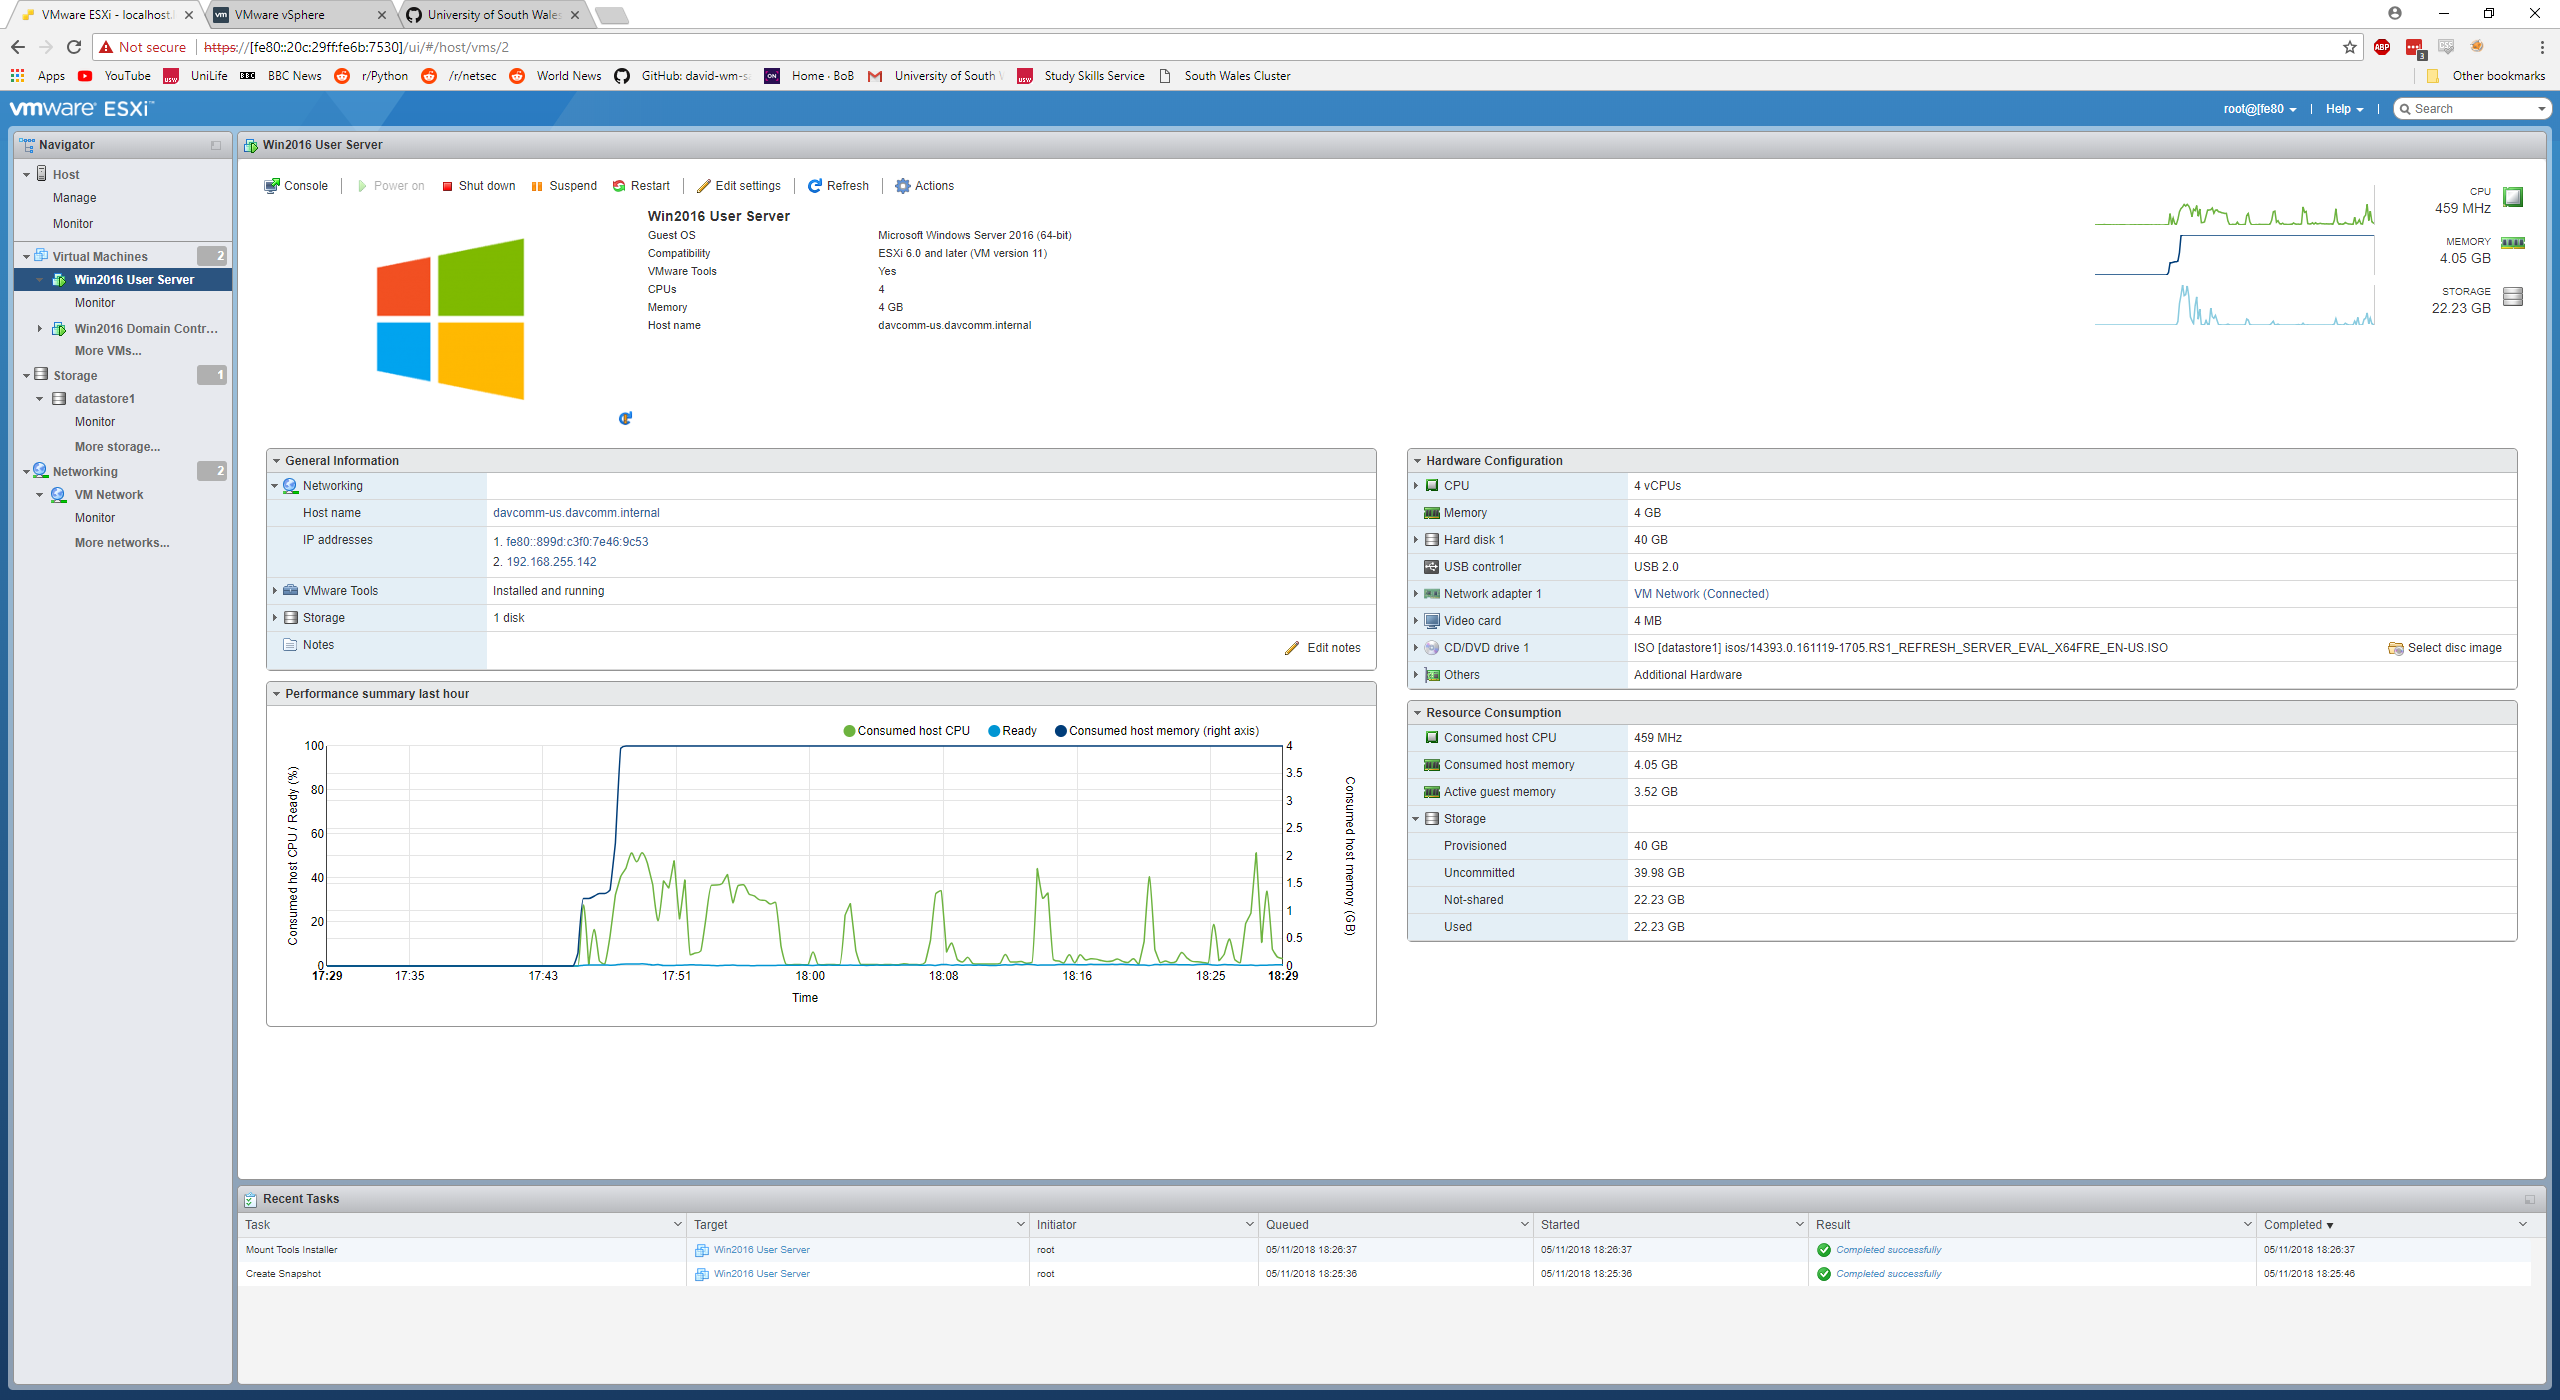
\includegraphics[width=\textwidth]{task2_9_winserver2016us_8}
  %     \caption{\todo{replace this with a proper figure description}}
  %     \label{fig:task2:vspherec_us8}
  %   \end{figure}
  \item In `Server Manager', select `Add roles and features' and under `File and Storage Services' select `File Server'.
    \begin{figure}[H]
      \centering
      \captionsetup{skip=2pt}
      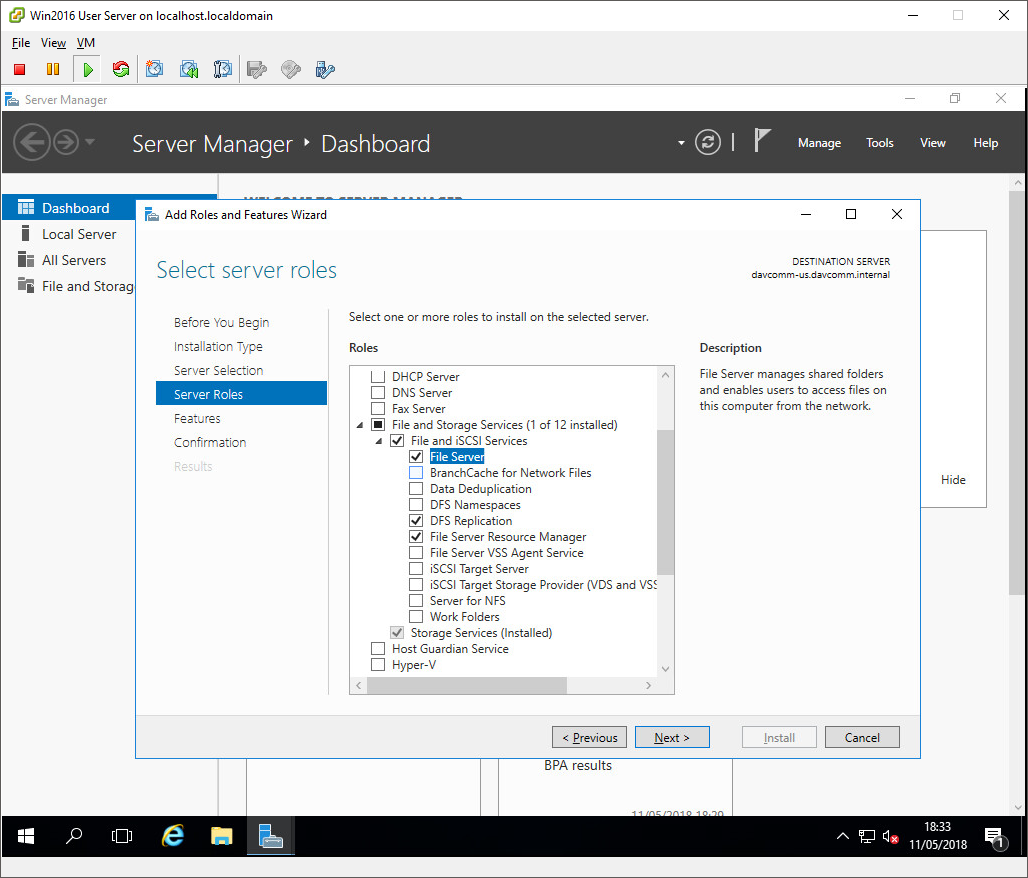
\includegraphics[width=\textwidth]{task2_9_winserver2016us_9}
      \caption{[2] Server 2016 US: Adding the `File Server' role}
      \label{fig:task2:vspherec_us9}
    \end{figure}
  % \item \todo{set failover clustering role}
  %   \begin{figure}[H]
  %     \centering
  %     \captionsetup{skip=2pt}
  %     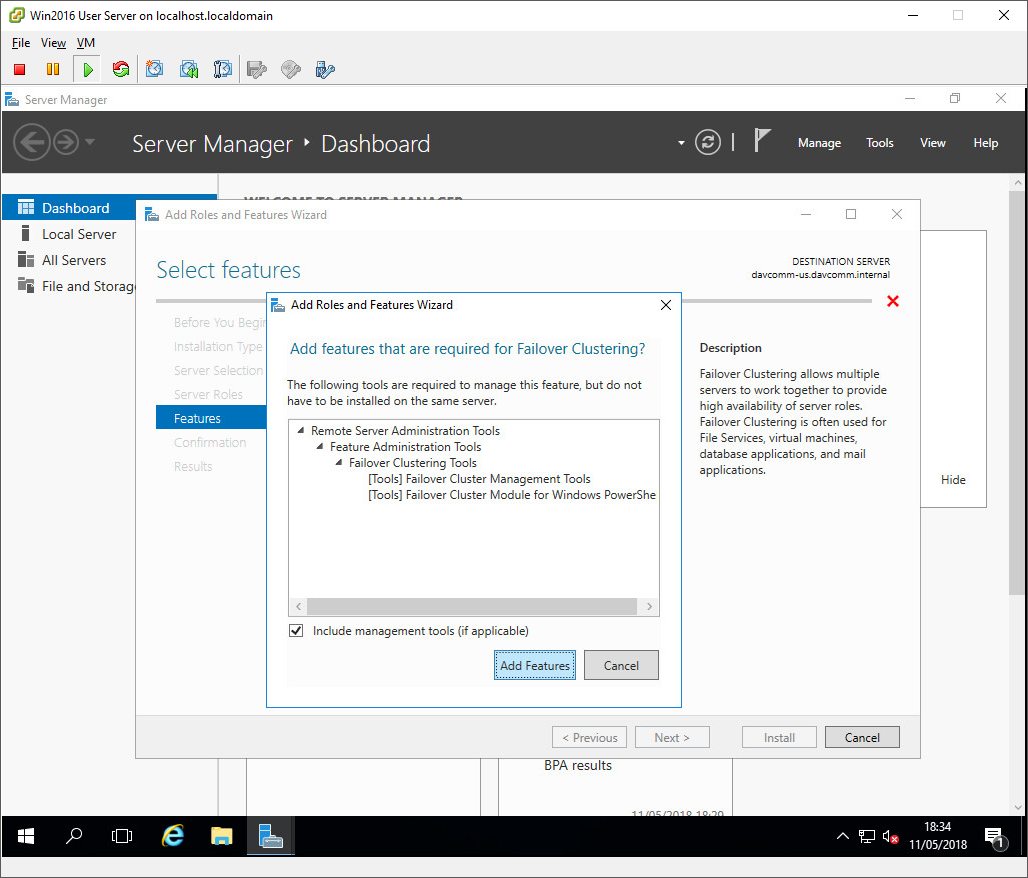
\includegraphics[width=\textwidth]{task2_9_winserver2016us_10}
  %     \caption{\todo{replace this with a proper figure description}}
  %     \label{fig:task2:vspherec_us10}
  %   \end{figure}
  \item Confirm the selections for the installation of roles on the User Server.
    \begin{figure}[H]
      \centering
      \captionsetup{skip=2pt}
      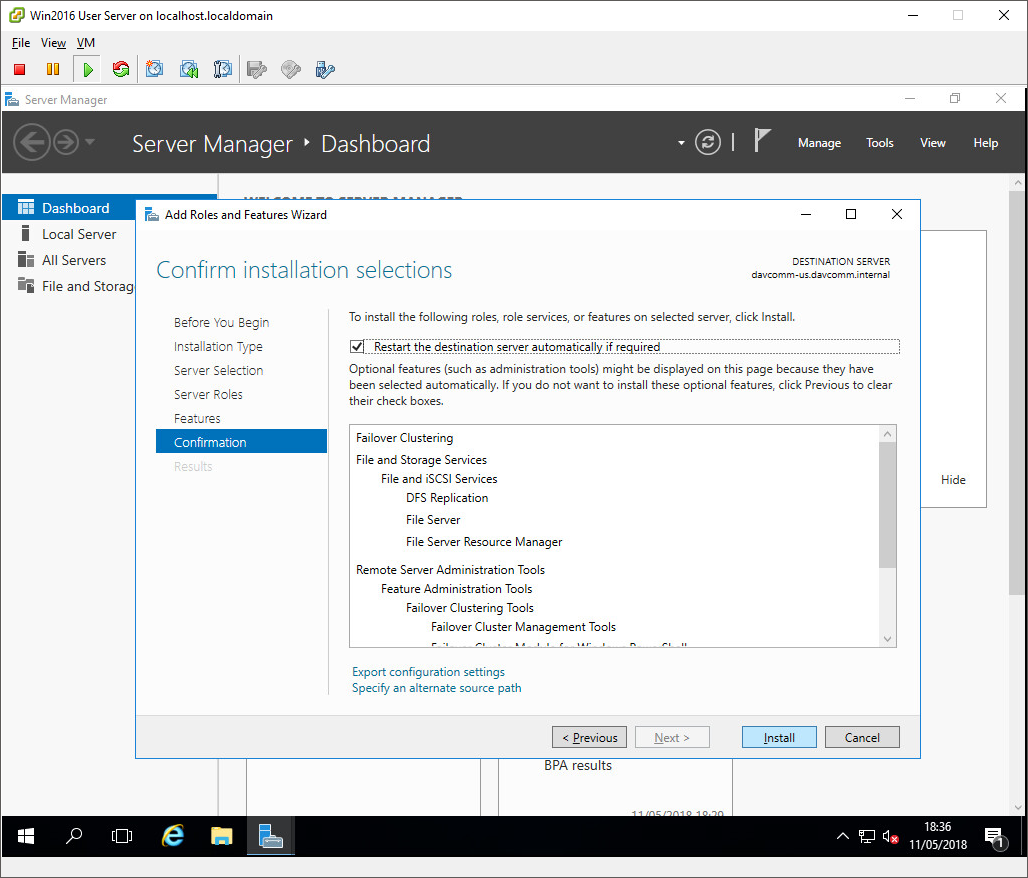
\includegraphics[width=\textwidth]{task2_9_winserver2016us_11}
      \caption{[2] Server 2016 US: Confirming the role selections}
      \label{fig:task2:vspherec_us11}
    \end{figure}
\end{enumerate}
\subsubsection{Set up a shared folder on the User Server}
\begin{enumerate}[series=task2methodology5]
  \item Open `Shares' under `File Storage and Services' and start the `New Share Wizard'.
    \begin{figure}[H]
      \centering
      \captionsetup{skip=2pt}
      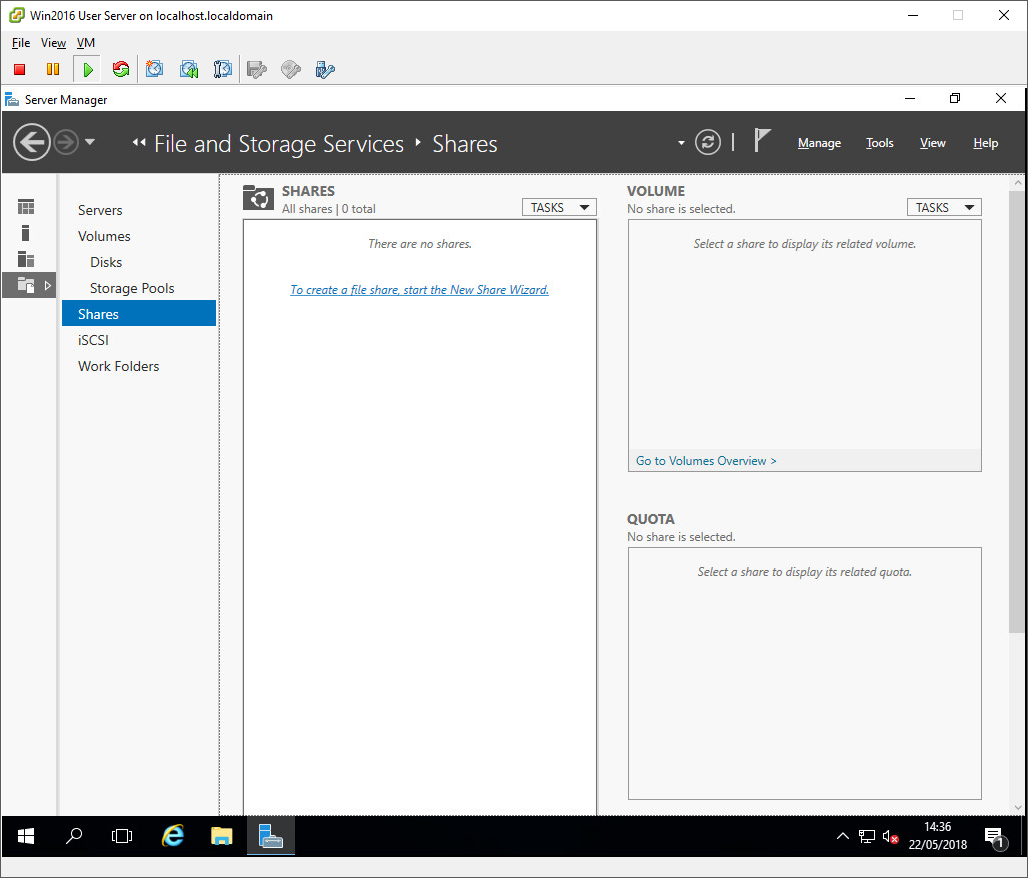
\includegraphics[width=\textwidth]{task2_9_winserver2016us_12_share01}
      \caption{[2] Server 2016 US: Starting the `New Share Wizard'}
      \label{fig:task2:vspherec_ussf01}
    \end{figure}
  \item Select `SMB Share - Quick'.
    \begin{figure}[H]
      \centering
      \captionsetup{skip=2pt}
      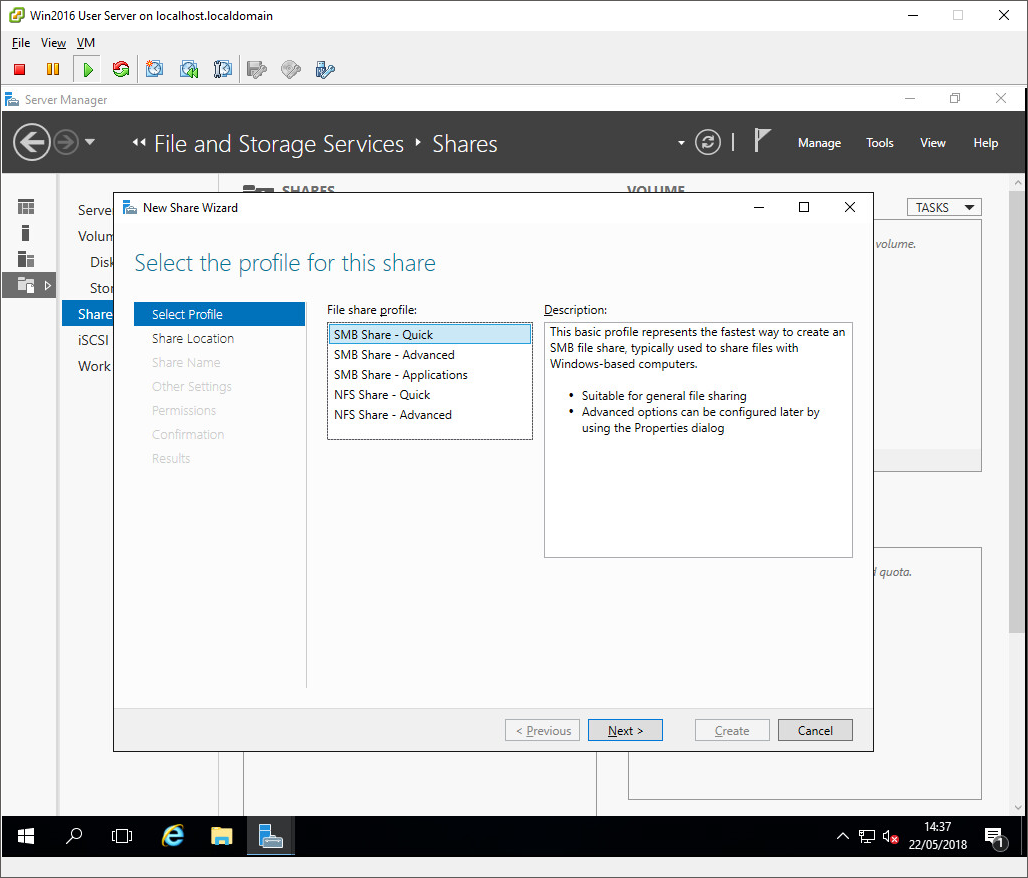
\includegraphics[width=\textwidth]{task2_9_winserver2016us_12_share02}
      \caption{[2] Server 2016 US: Selecting `SMB Share - Quick'}
      \label{fig:task2:vspherec_ussf02}
    \end{figure}
  \item Create a custom path to a location for the new share.
    \begin{figure}[H]
      \centering
      \captionsetup{skip=2pt}
      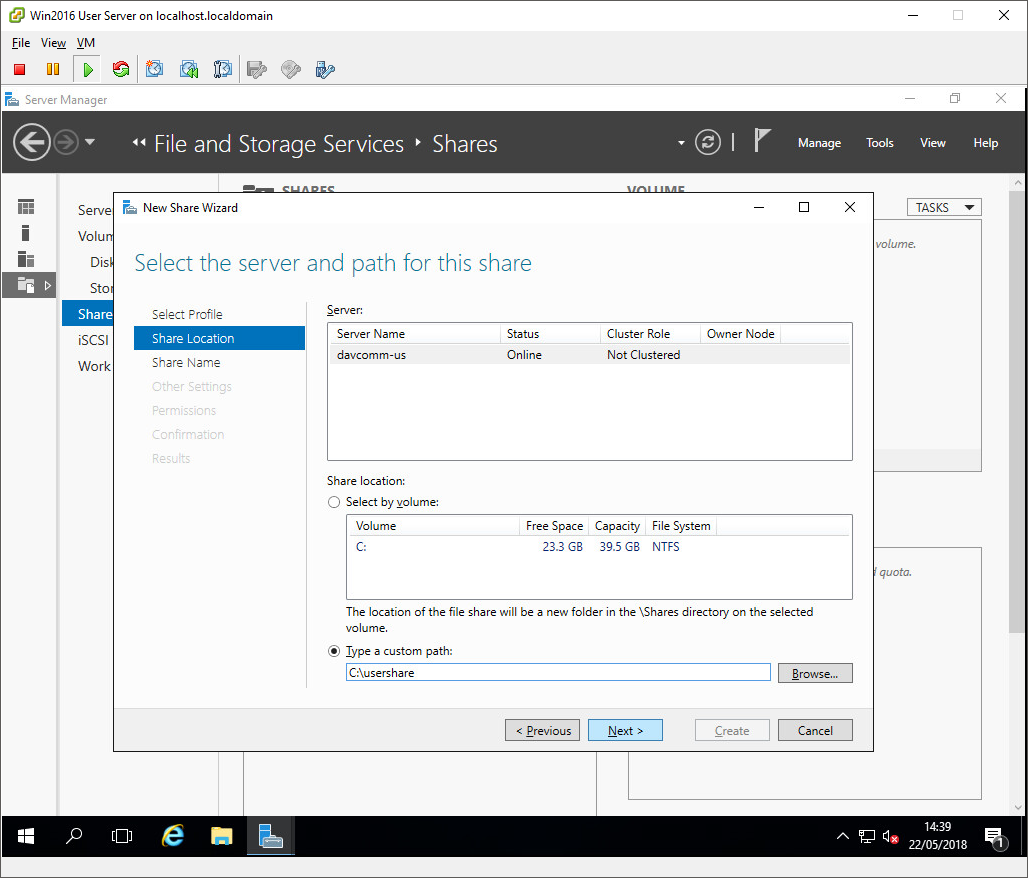
\includegraphics[width=\textwidth]{task2_9_winserver2016us_12_share04}
      \caption{[2] Server 2016 US: Setting the `Share Location' for the new share}
      \label{fig:task2:vspherec_ussf04}
    \end{figure}
  \item Tick the boxes to `Enable access-based enumeration' and `Encrypt data access'.
    \begin{figure}[H]
      \centering
      \captionsetup{skip=2pt}
      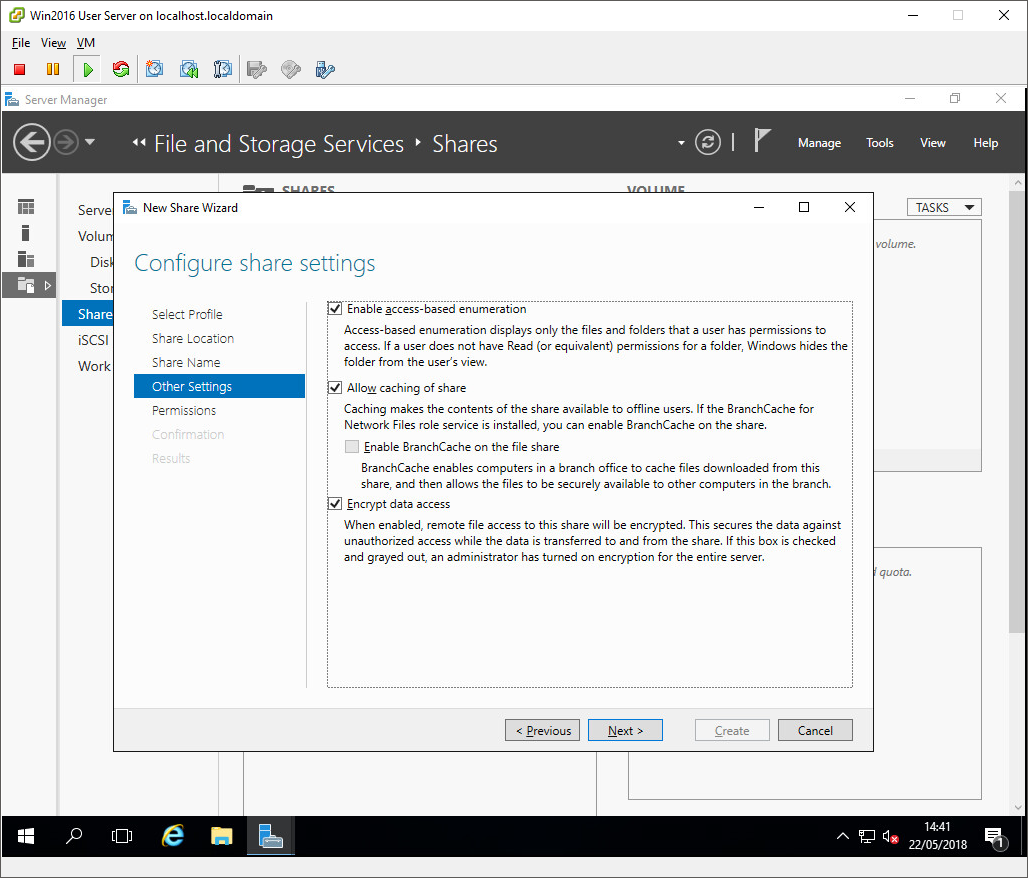
\includegraphics[width=\textwidth]{task2_9_winserver2016us_12_share06}
      \caption{[2] Server 2016 US: Configuring settings for the new share}
      \label{fig:task2:vspherec_ussf06}
    \end{figure}
  \item Customise permissions for the new share. This entails disabling inheritance and then modifying the two Users principals to apply to `This folder only'. Once this is done, the two Users principals will merge to be a single Users principal.
    \begin{figure}[H]
      \centering
      \captionsetup{skip=2pt}
      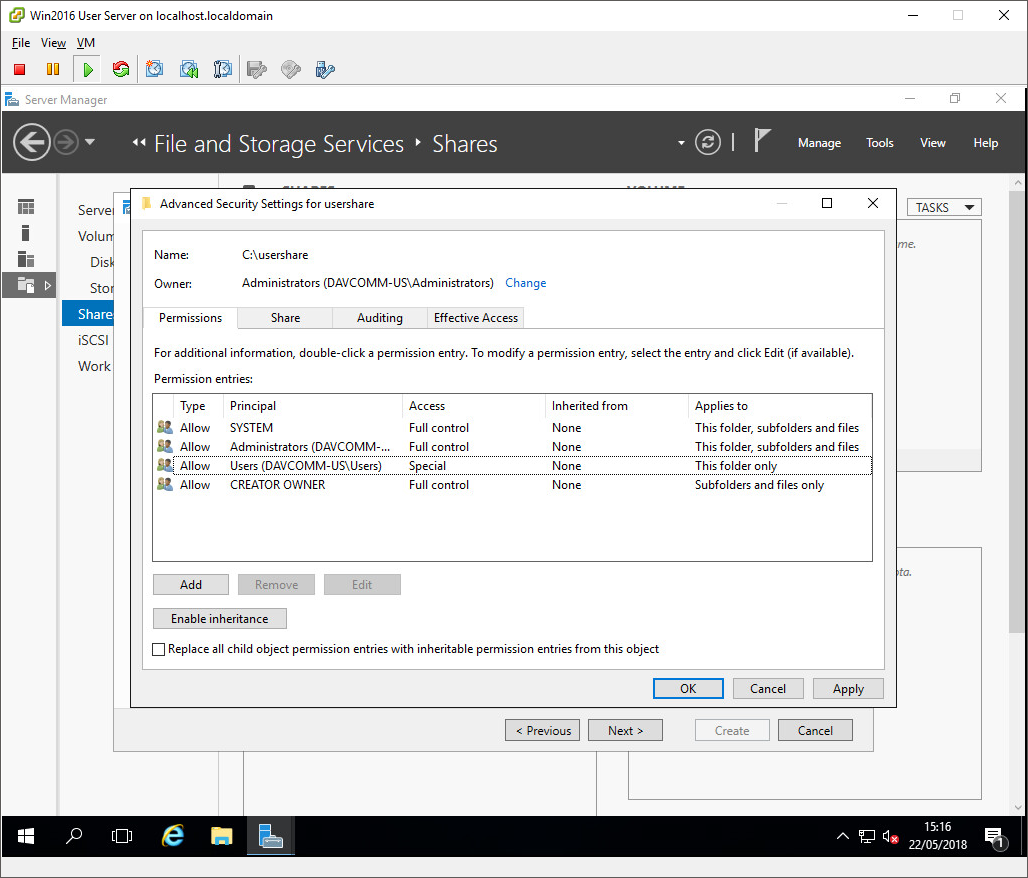
\includegraphics[width=\textwidth]{task2_9_winserver2016us_12_share07}
      \caption{[2] Server 2016 US: Customising permissions for the new share}
      \label{fig:task2:vspherec_ussf07}
    \end{figure}
    \begin{figure}[H]
      \centering
      \captionsetup{skip=2pt}
      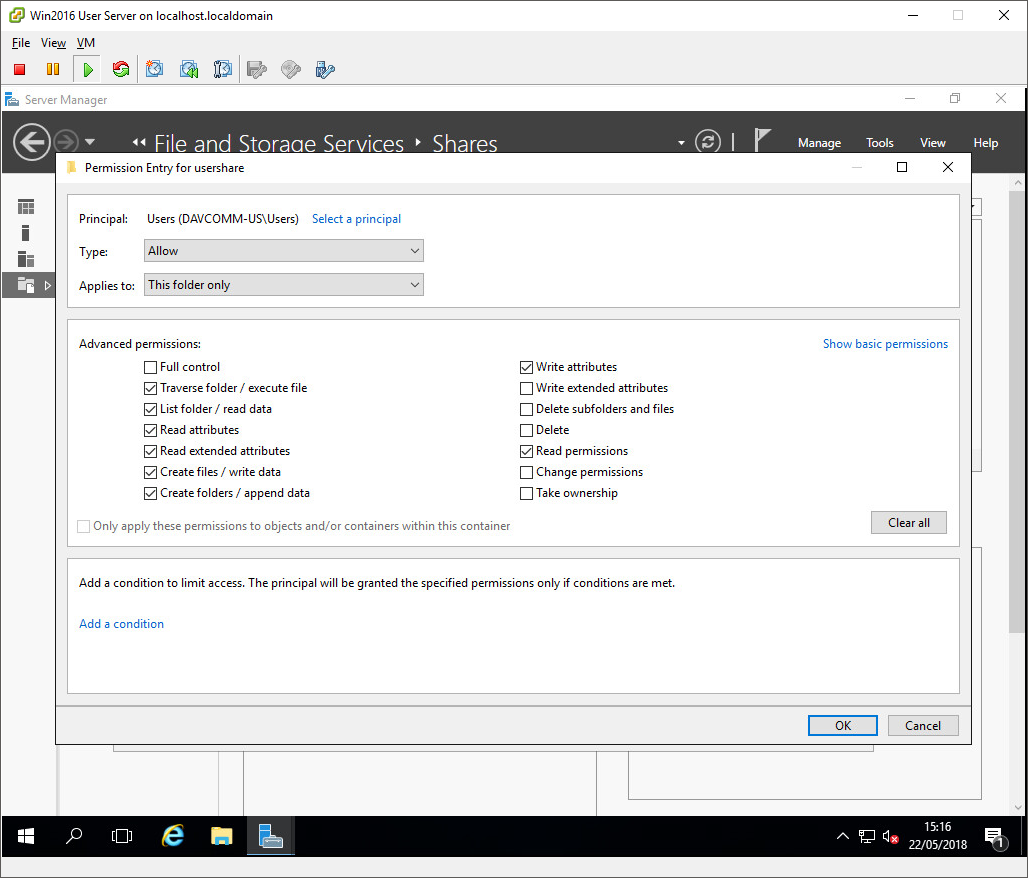
\includegraphics[width=\textwidth]{task2_9_winserver2016us_12_share08}
      \caption{[2] Server 2016 US: Modifying advanced permissions for the new share}
      \label{fig:task2:vspherec_ussf08}
    \end{figure}
  \item \todo{damn, the client doesn't exist until task 3 is done} Once this is done, step through the rest of the wizard to review the settings adjusted and then confirm the creation of the new share.
    \begin{figure}[H]
      \centering
      \captionsetup{skip=2pt}
      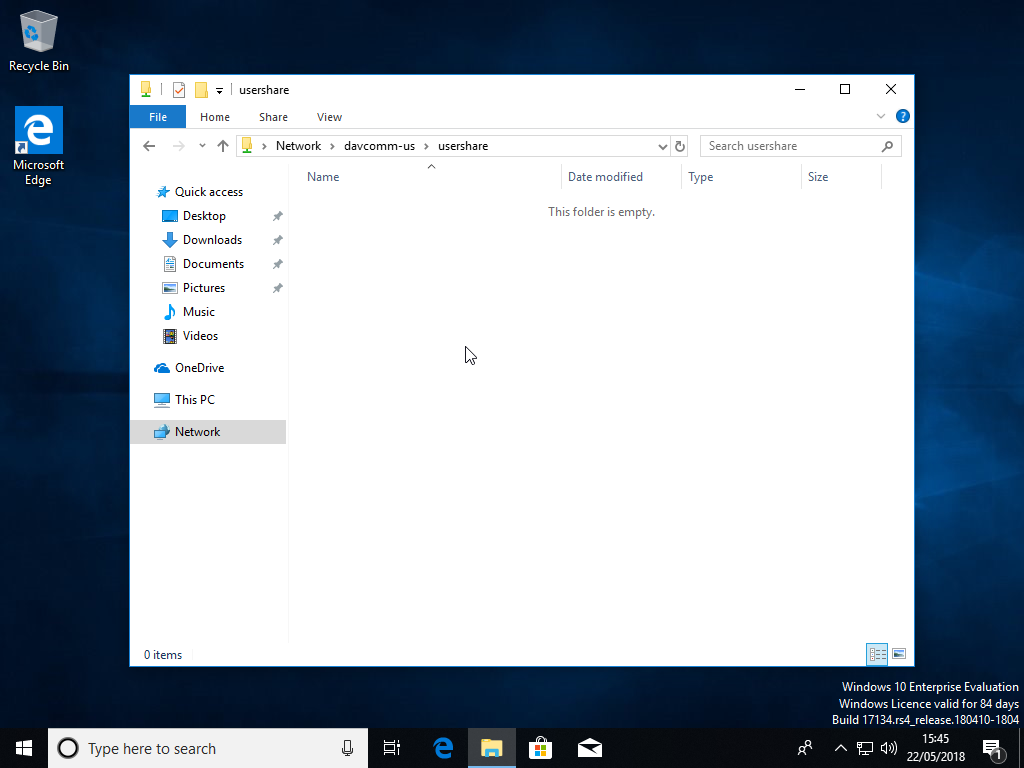
\includegraphics[width=\textwidth]{IY1D403_Windows_10_x64_Client-2018-05-22-15-46-11}
      \caption{[2] Windows 10 Client: Checking that the client can see the new share}
      \label{fig:task2:vspherec_ussfx}
    \end{figure}
  \item \todo{damn, the client doesn't exist until task 3 is done} By attempting to access the shared folder of user `skywrath' from the user `lich', it can be seen that the security configuration (access-based enumeration) has been configured correctly.
    \begin{figure}[H]
      \centering
      \captionsetup{skip=2pt}
      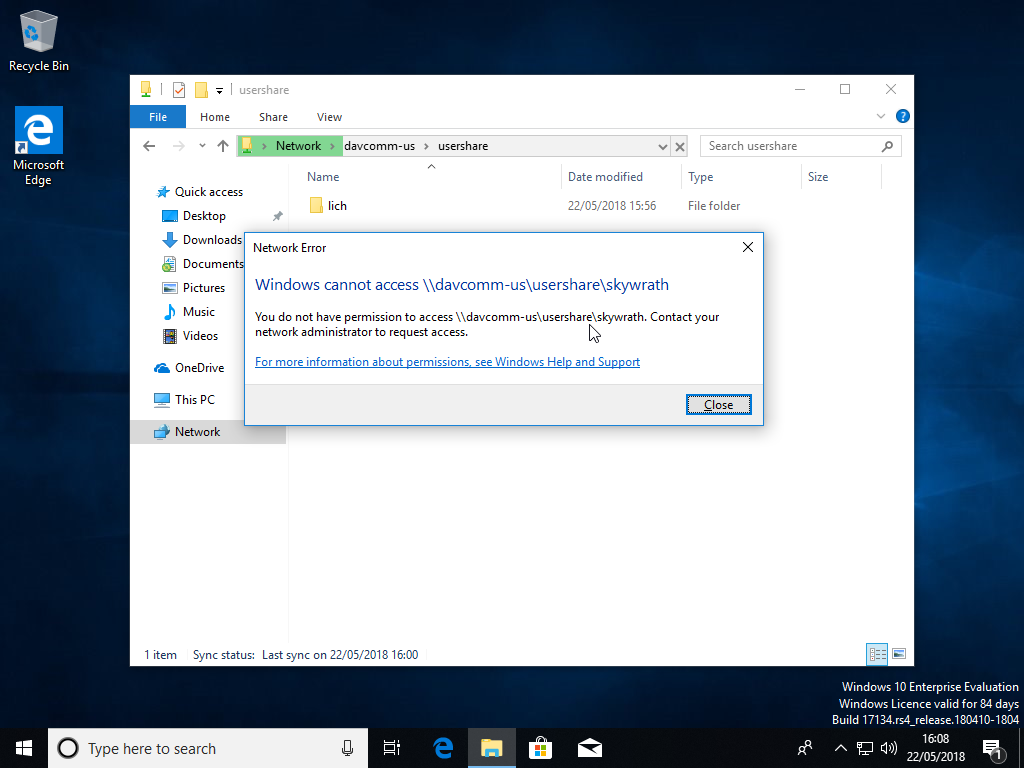
\includegraphics[width=\textwidth]{IY1D403_Windows_10_x64_Client-2018-05-22-16-08-20}
      \caption{[2] Windows 10 Client: Checking that the share is secured correctly}
      \label{fig:task2:vspherec_ussfx2}
    \end{figure}
\end{enumerate}
% \subsubsection{\todo{Create a failover configuration}}
% \todo{ahhhhh, how? \url{https://docs.vmware.com/en/VMware-vSphere/6.0/vsphere-esxi-vcenter-server-601-setup-mscs.pdf}}
